\chapter{Desenvolvimento}
\vspace{-2.5 cm}

% Este Capítulo apresenta o que foi desenvolvido até o momento.
Este Capítulo apresenta o que foi desenvolvido como resultado deste trabalho,
visando alcançar os objetivos propostos.

\section{O simulador Simiam e alterações necessárias}

O Simulador Simiam foi implementado pela Universidade Georgia Tech, 
inicialmente oferecendo apenas suporte ao robô Khepera 3. Posteriormente, 
para atender necessidades do curso \textit{Control of Mobile Robots}, hospedado 
na plataforma ``Coursera.org'', o robô de baixo custo QuickBot foi adicionado. 
Os robôs Khepera e QuickBot reais podem ser vistos na Figura \ref{fig:RobosK3QB}. 
Suas contrapartes simuladas estão retratadas na Figura \ref{fig:RobosEmSimulador}.

O curso mencionado foi removido da plataforma no dia 17 de Agosto de 2020 e apenas
os alunos concluíntes possuem acesso. De qualquer forma, o simulador ainda pode ser
obtido gratuitamente.

\begin{figure}[ht]
\centering
\caption{Robôs Khepera 3 e QuickBot}
\label{fig:RobosK3QB}
	\begin{subfigure}[b]{0.49\textwidth}%
		\centering
		% fbox{}
		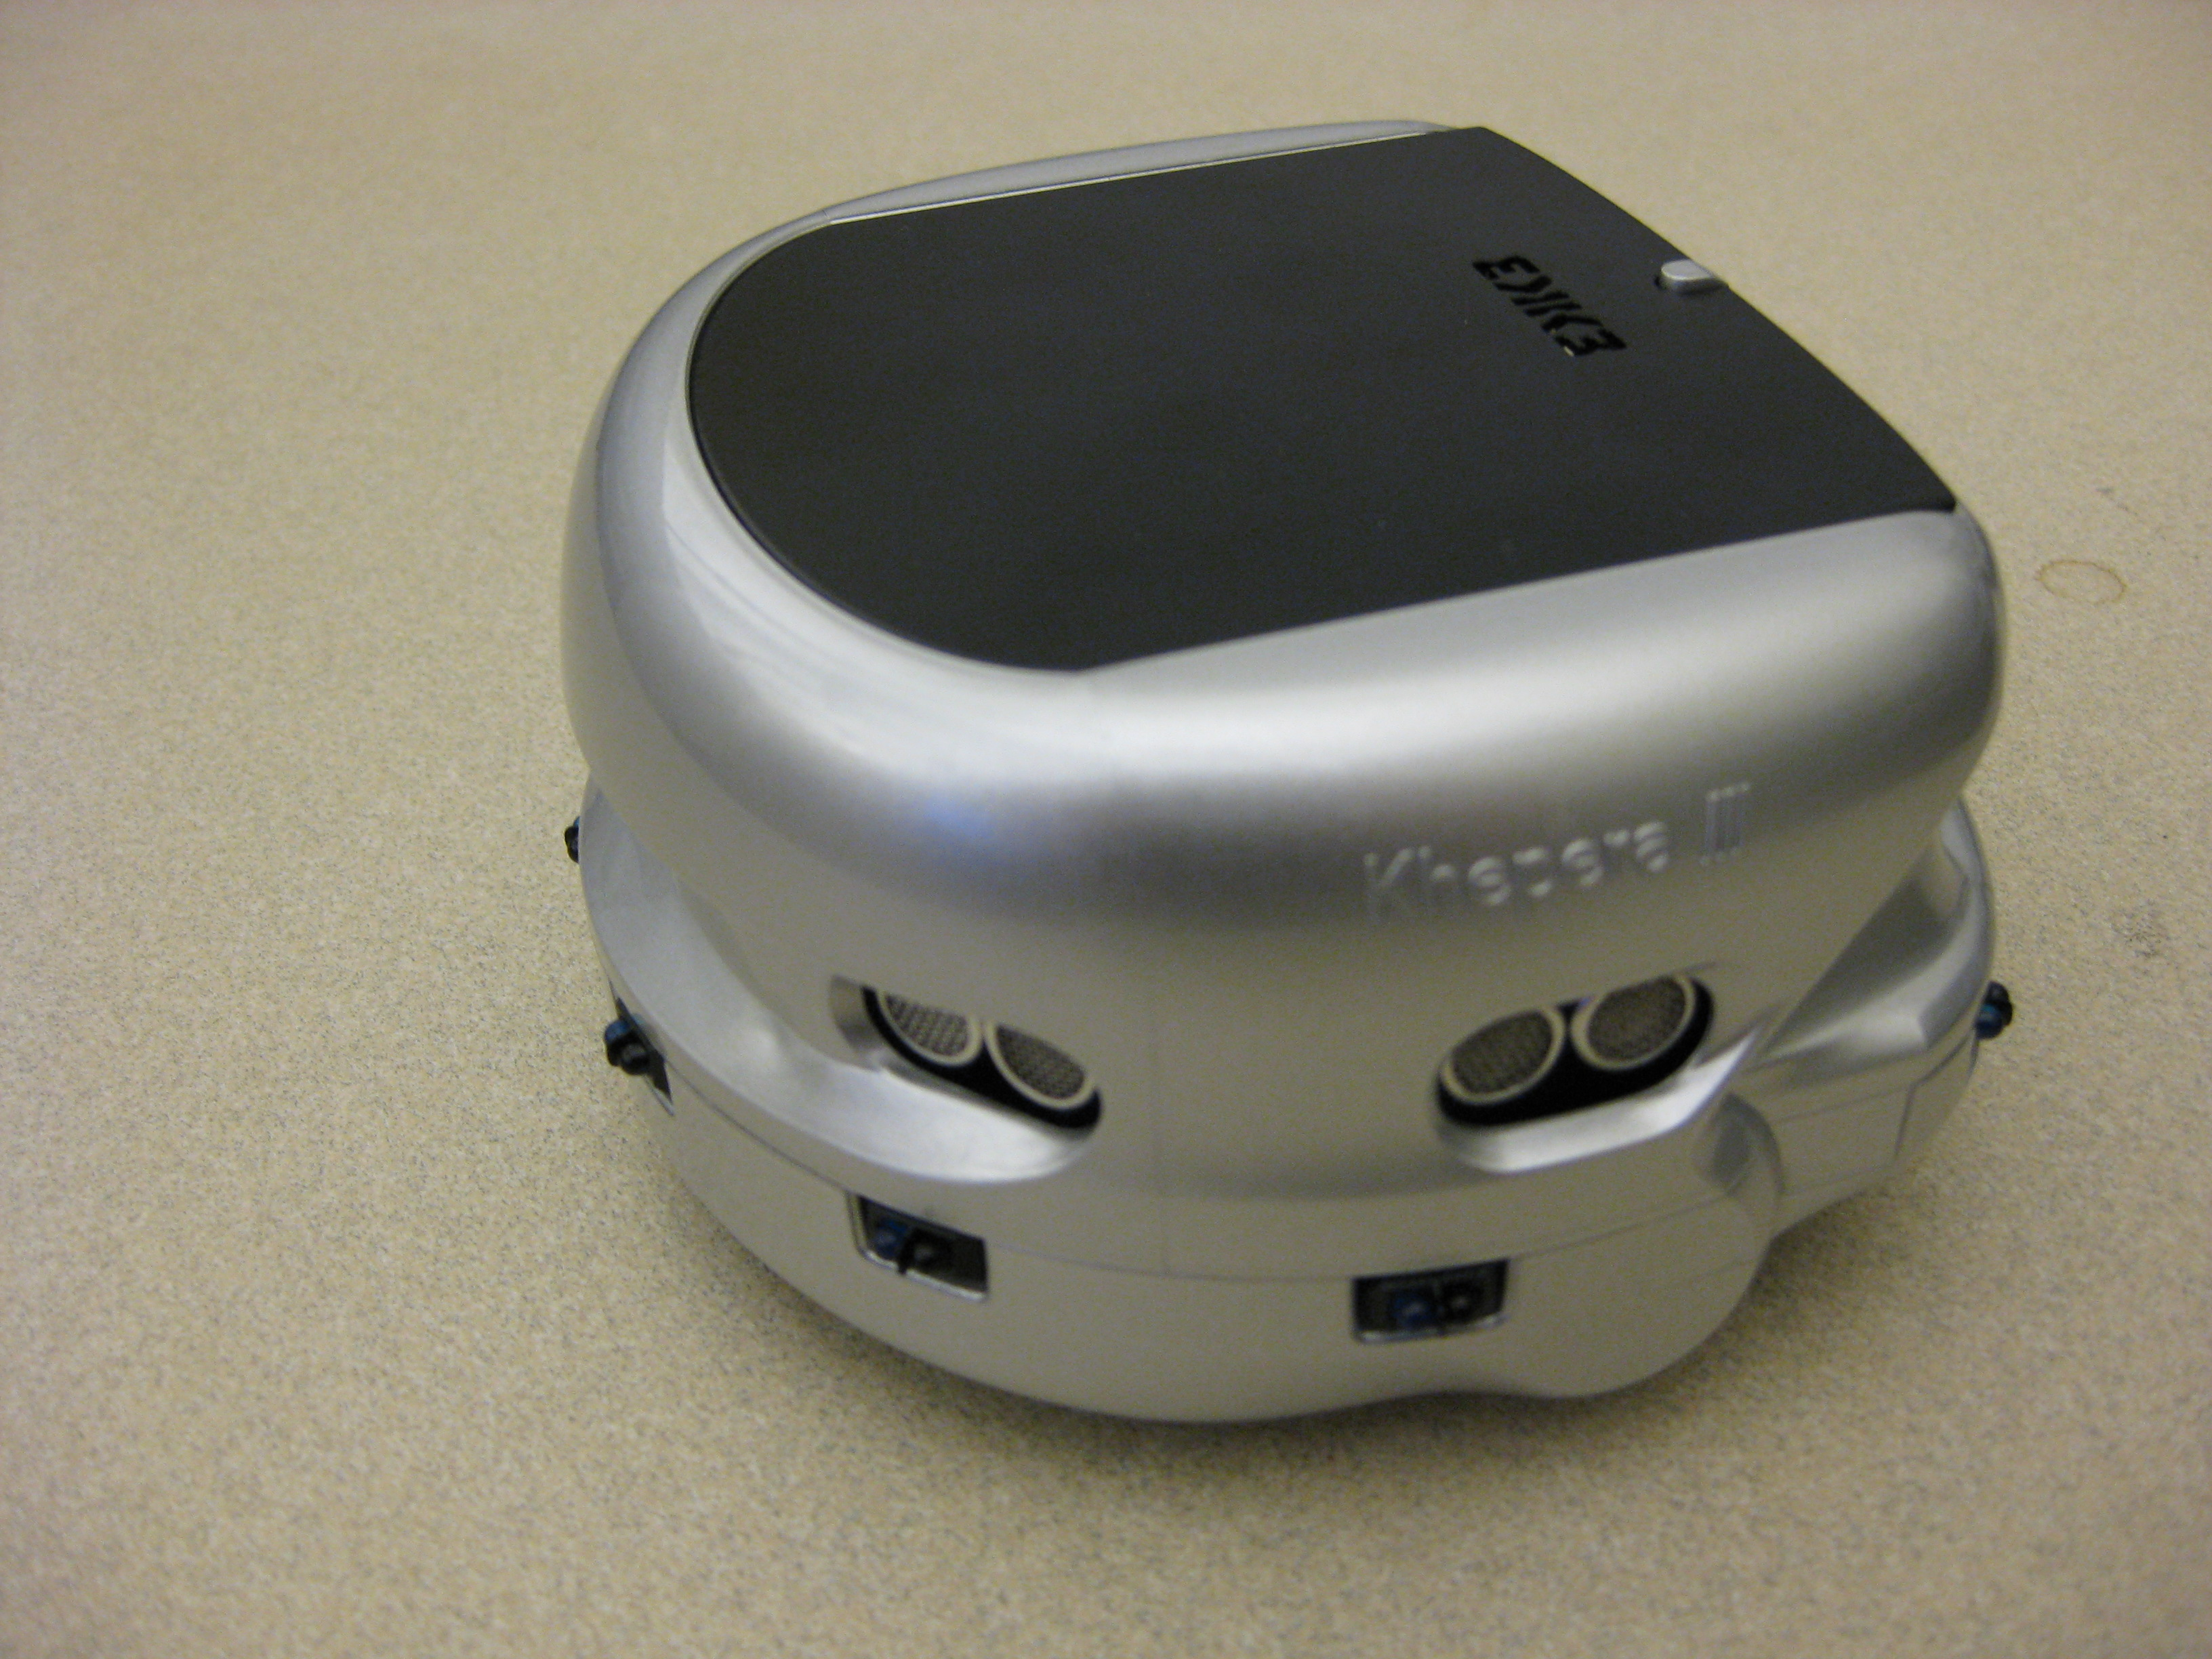
\includegraphics[trim= 8cm 0cm 0cm 0cm,clip,
scale=0.14]{Figuras/Khepera_III_robot}
		\subcaption{Robô Khepera 3}
	  	\label{fig:test1}
	\end{subfigure}
	~
	\begin{subfigure}[b]{0.49\textwidth}%
		\centering
		% fbox{}
		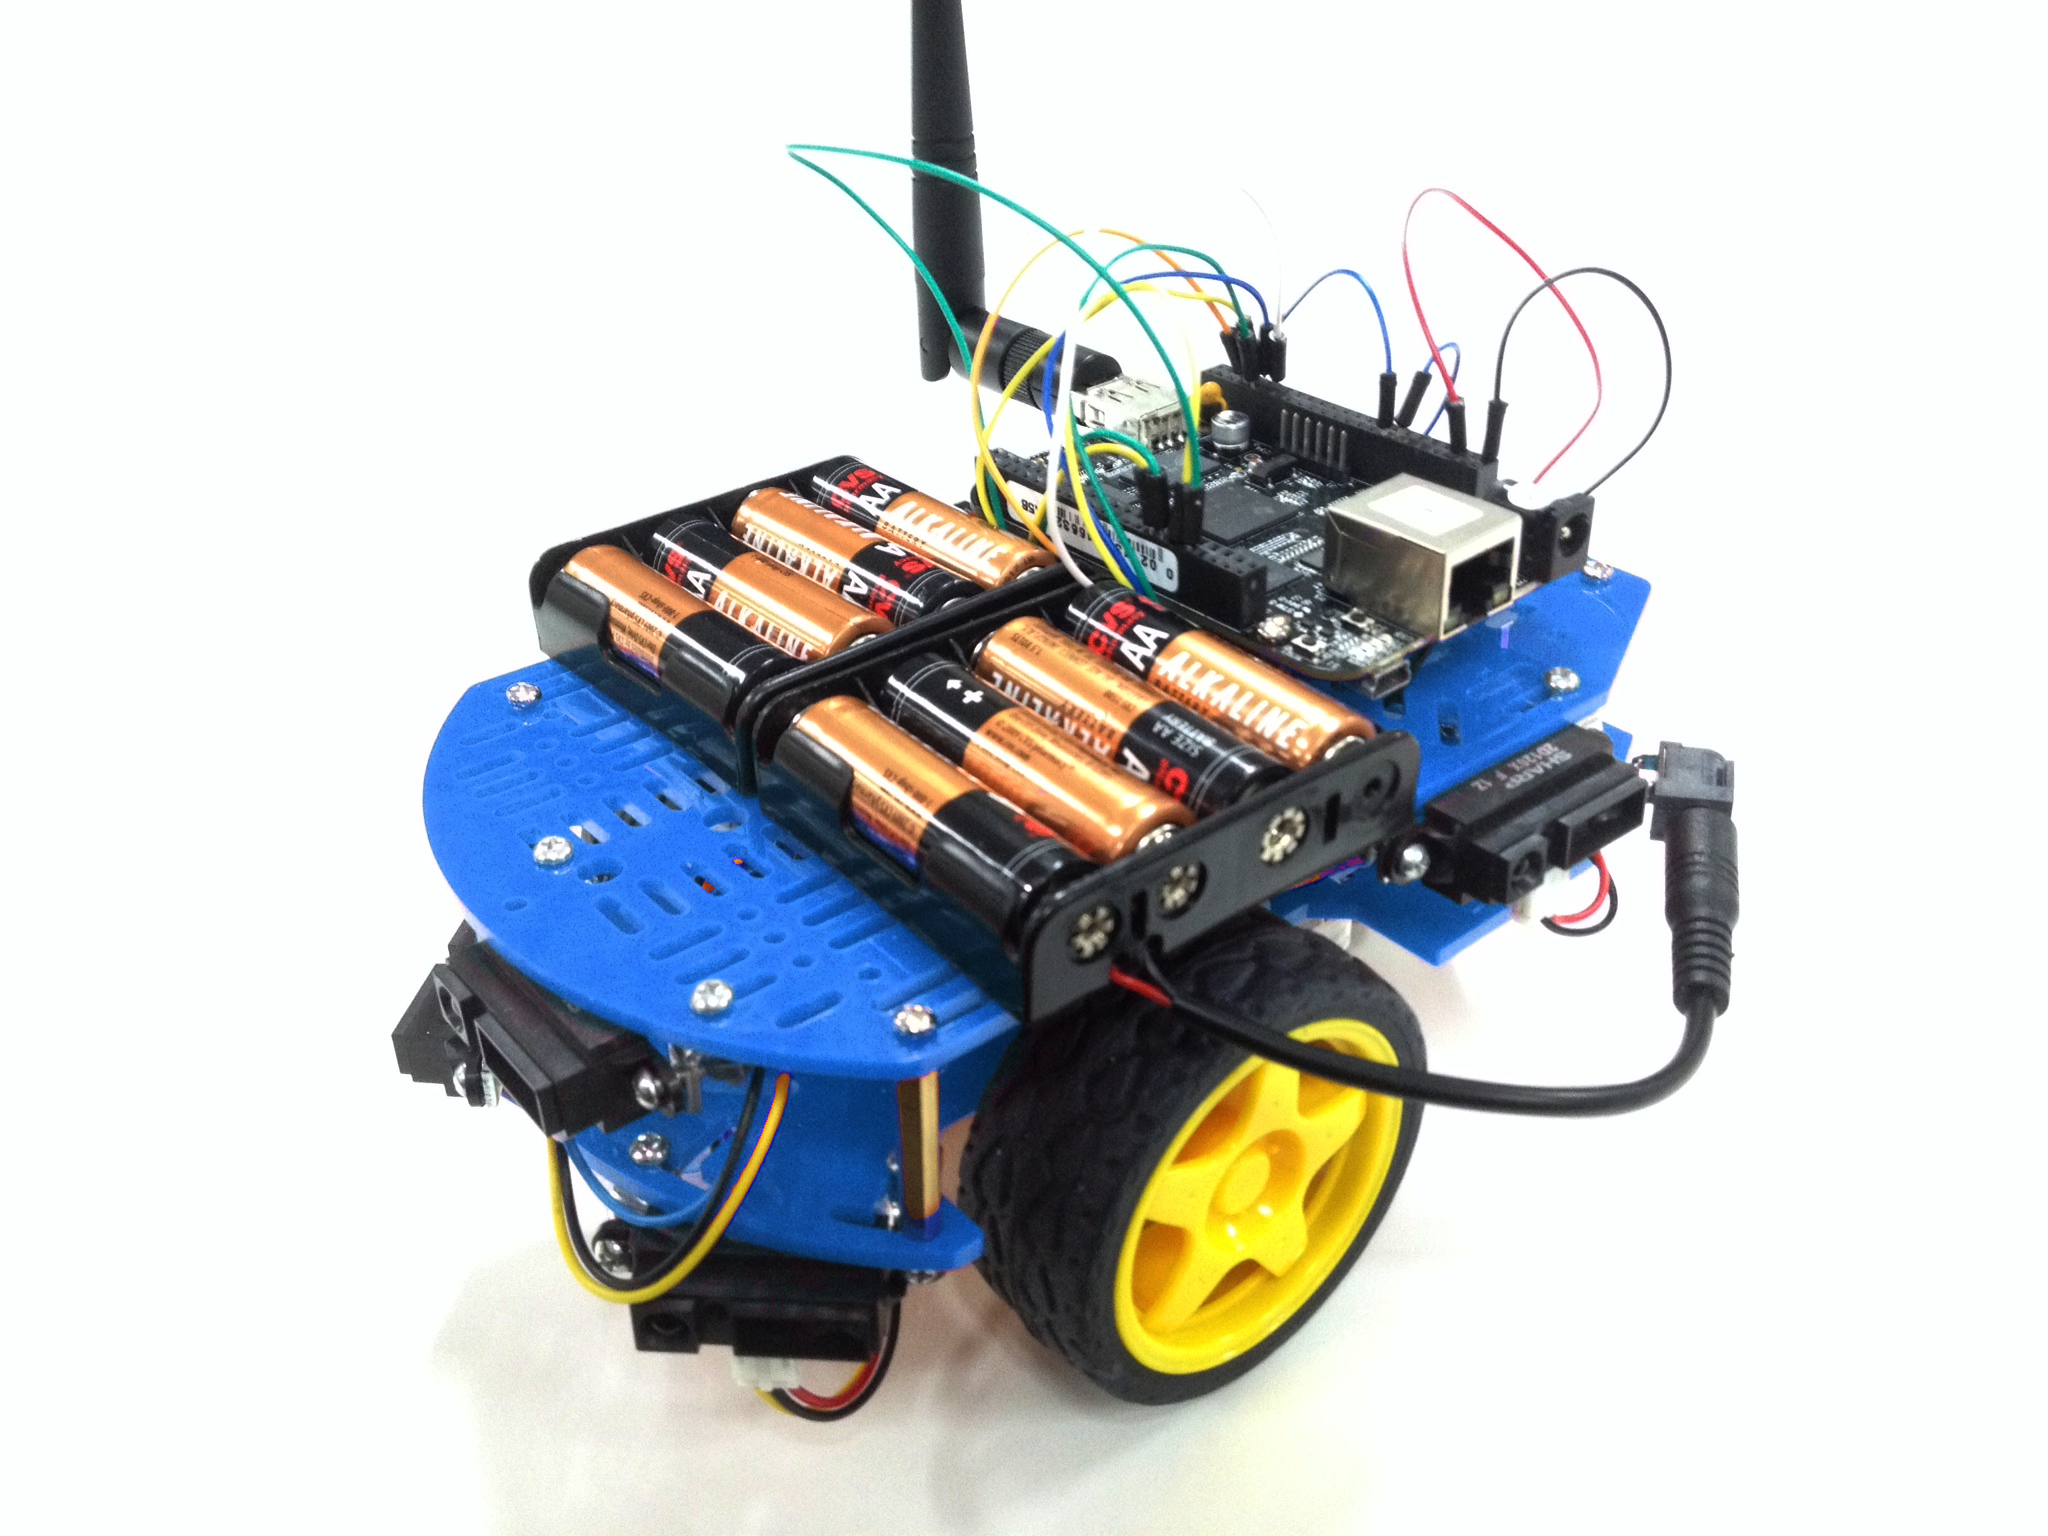
\includegraphics[trim={6cm 0cm 3cm 0cm},clip,
scale=0.09]{Figuras/quickbot-blue}
		\subcaption{Robô QuickBot}
	  	\label{fig:test2}
	\end{subfigure}
	
	\textbf{Fonte: \citeonline{im:Khepera}, \citeonline{im:QuickBot_Blue}}
\end{figure}


%		\begin{figure}[!htb]
%			\centering
%			\caption{Robôs Khepera e QuickBot fisicamente e em simulação}
%			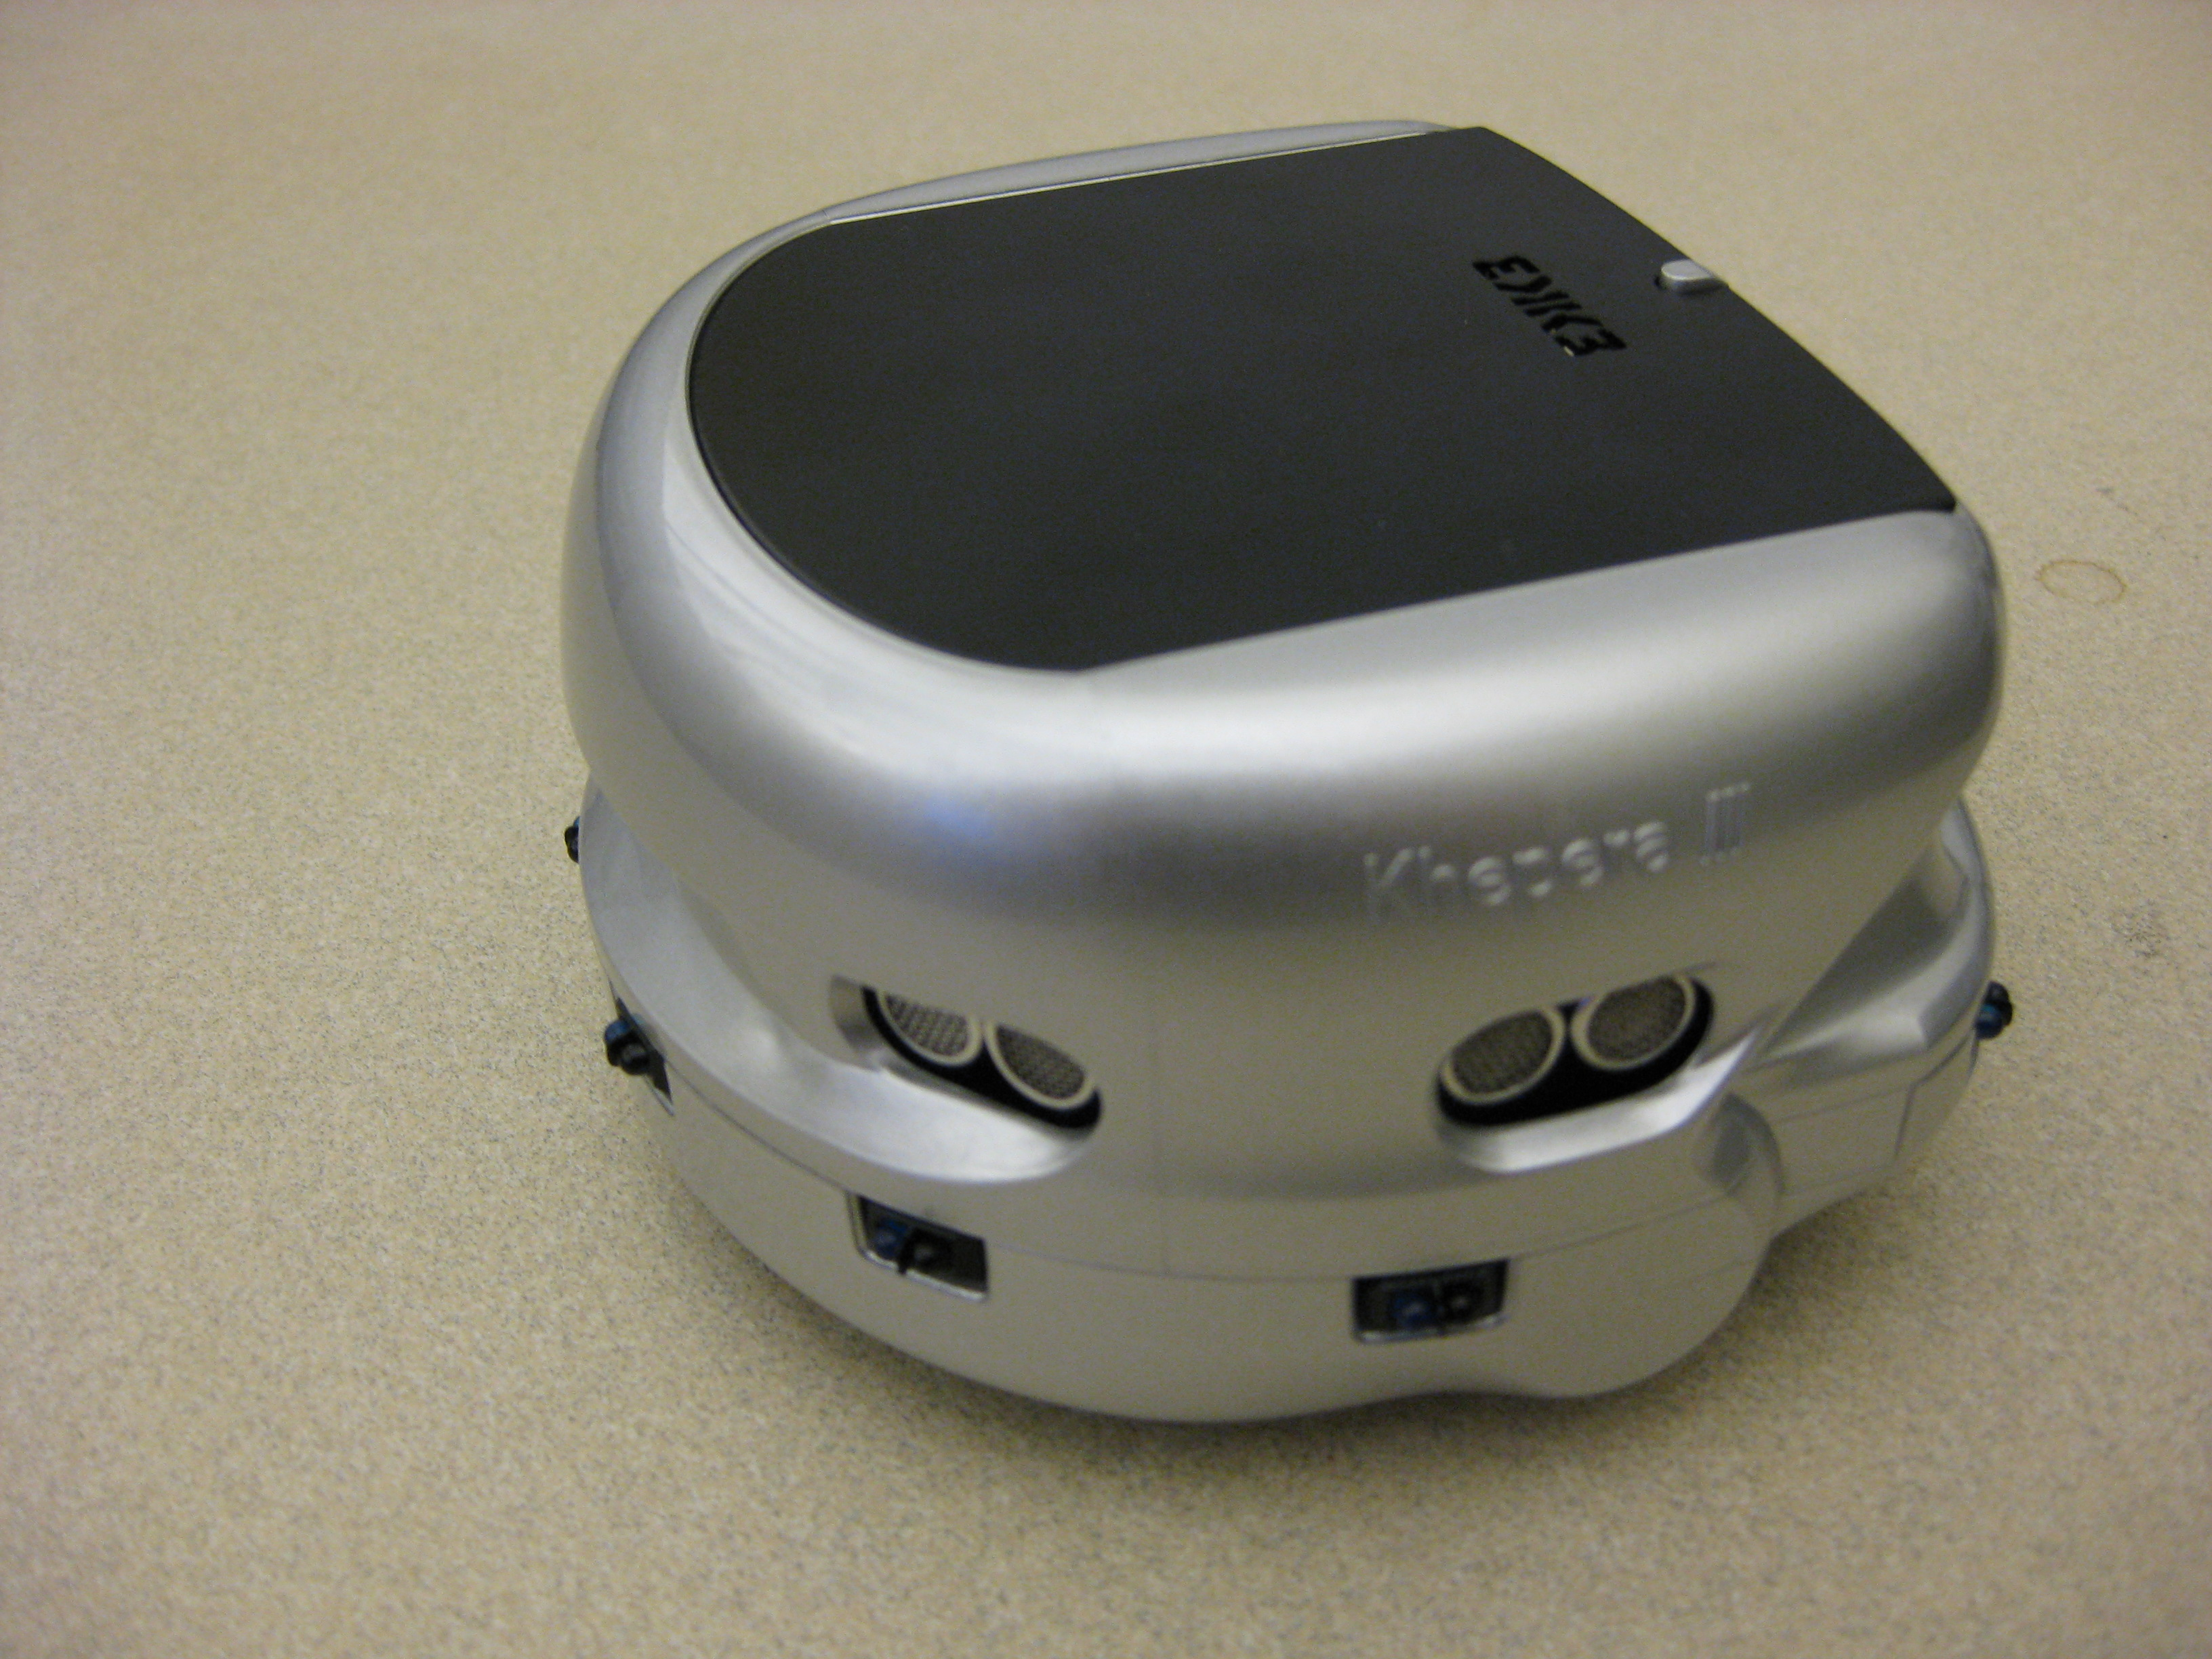
\includegraphics[trim={0cm 0cm 0cm 0cm},clip,
%scale=0.35]{Figuras/Khepera_III_robot}
%			%\vspace{-0.4cm}
%			\label{fig:RobosESim}
%		\end{figure}

%		\begin{figure}[!htb]
%			\centering			
%			\caption{Robôs Khepera e QuickBot fisicamente e em simulação}
%			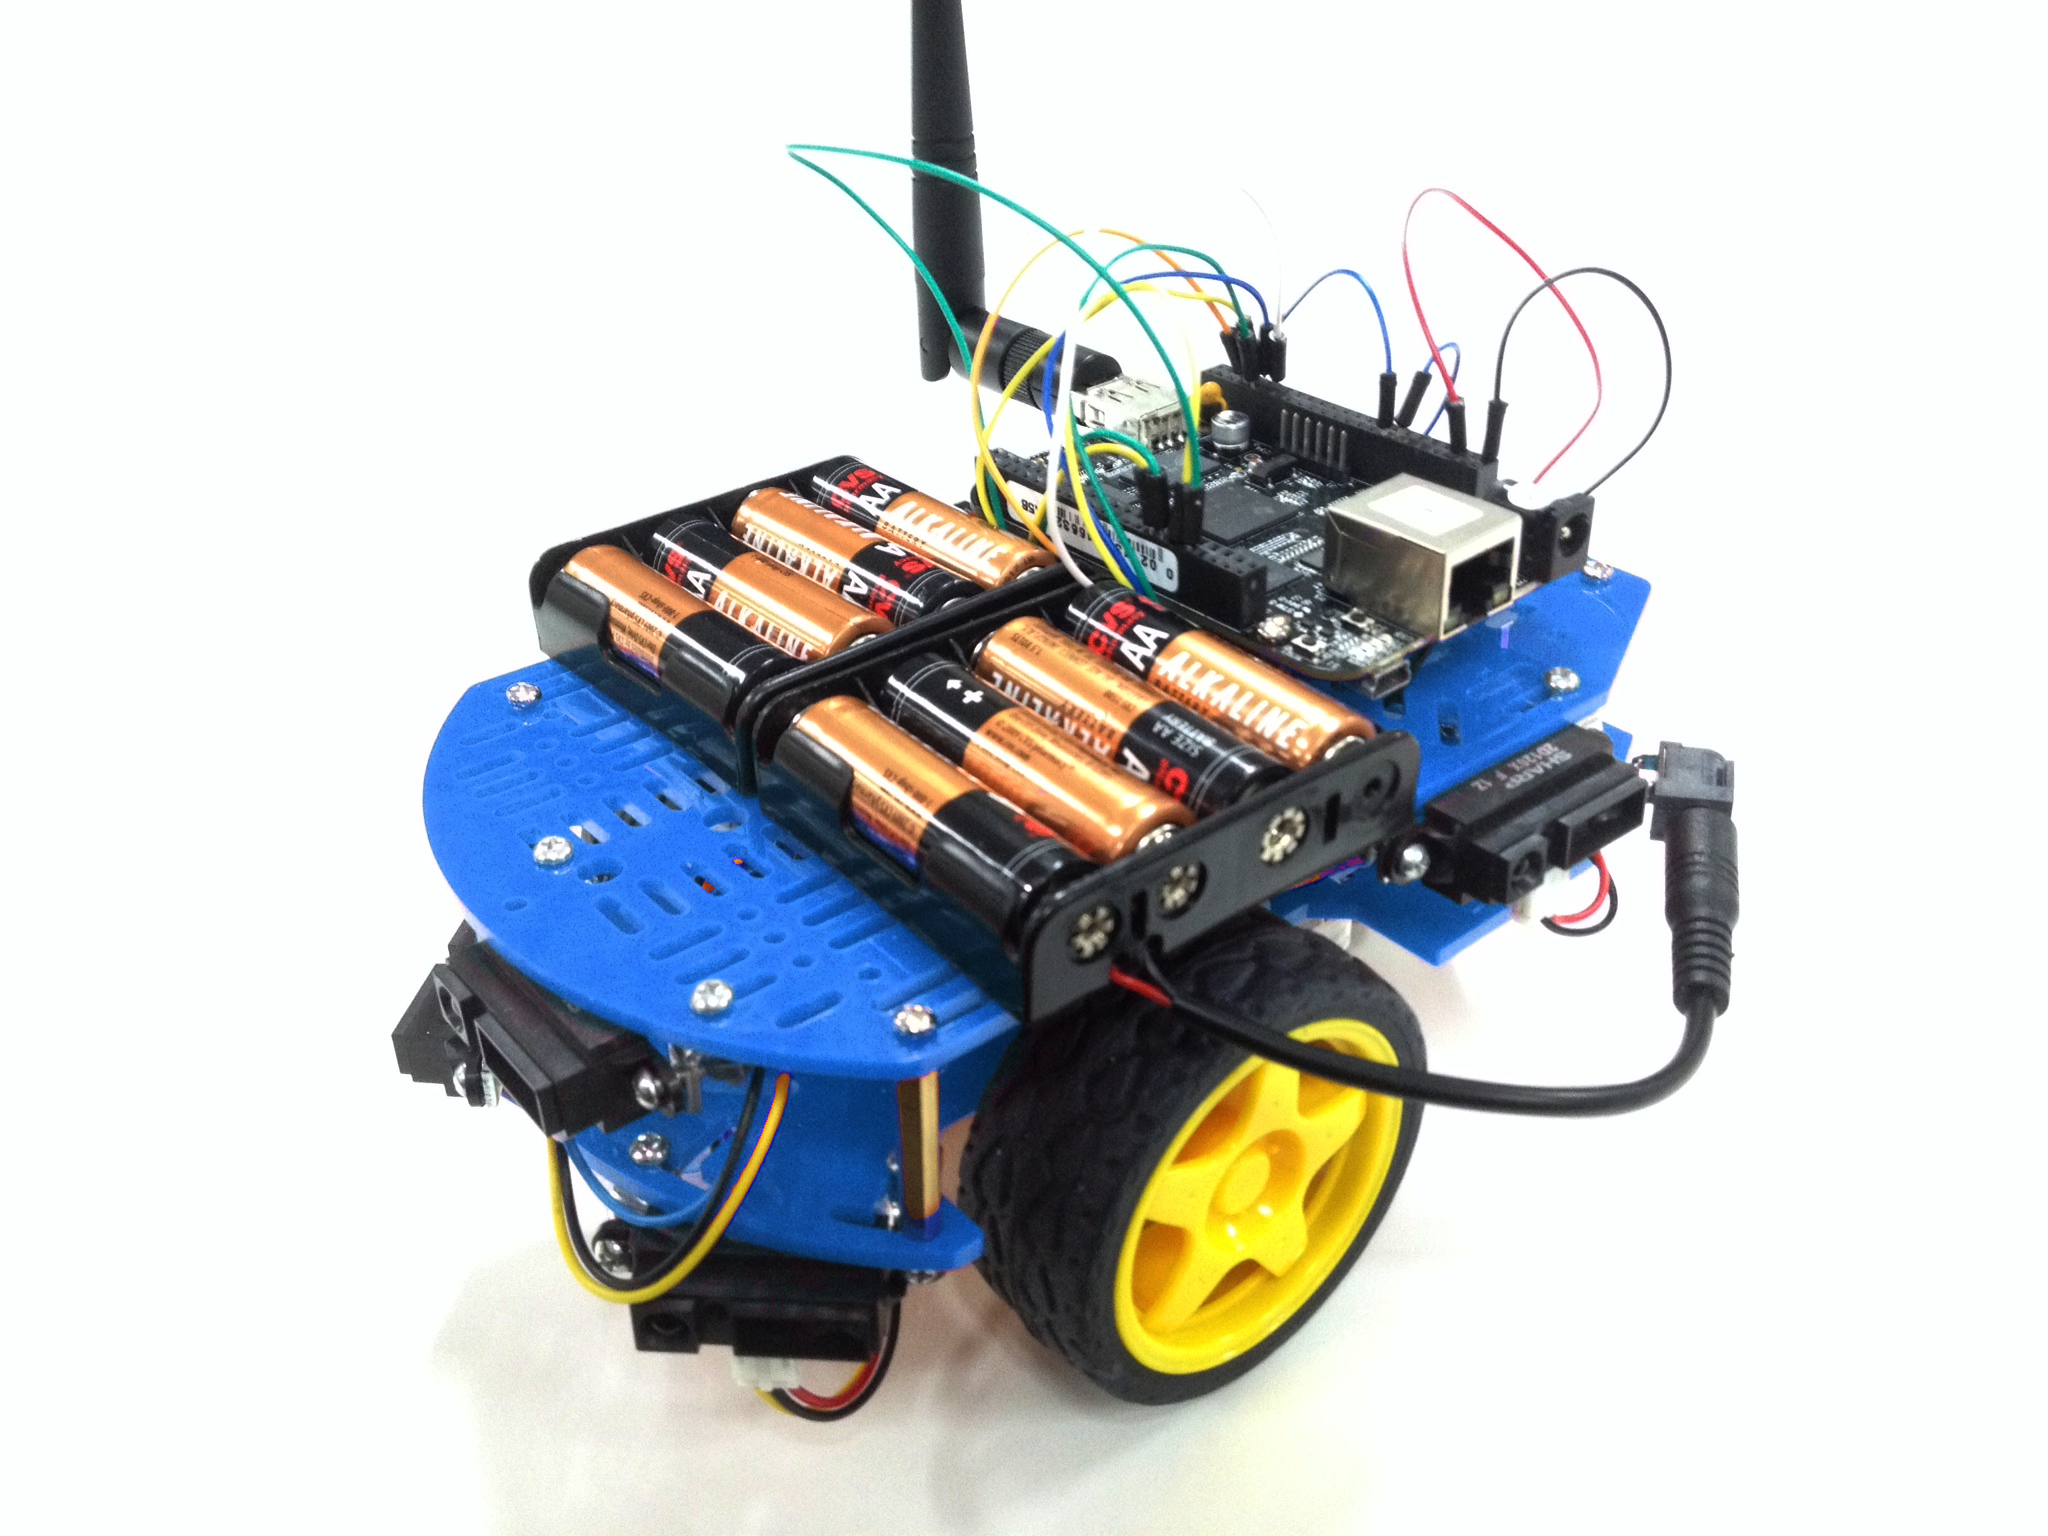
\includegraphics[trim={0cm 0cm 0cm 0cm},clip,
%scale=0.25]{Figuras/quickbot-blue}
%			%\vspace{-0.4cm}
%			\label{fig:RobosESim}
%		\end{figure}

%		\begin{figure}[!htb]
%			\centering
%			\caption{Robôs Khepera e QuickBot fisicamente e em simulação}
%			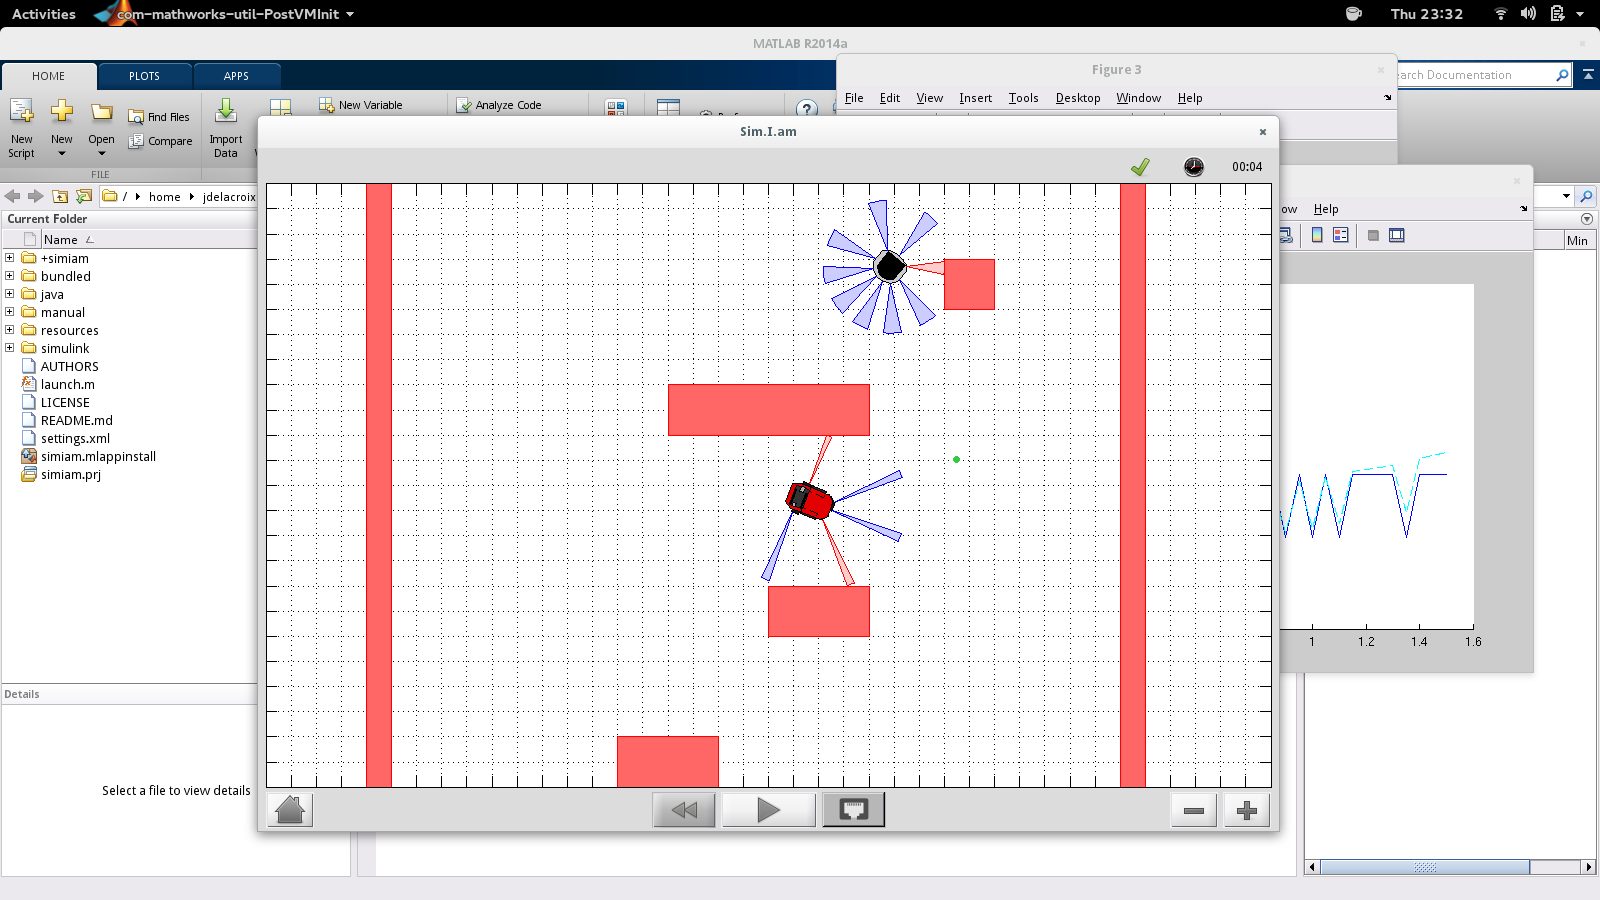
\includegraphics[trim={0cm 0cm 0cm 0cm},clip,
%scale=0.25]{Figuras/simiam-screenshot}
%			%\vspace{-0.4cm}
%			\label{fig:RobosESim}
%		\end{figure}


%\begin{figure}
%\begin{minipage}[c][11cm][t]{.5\textwidth}
%  \vspace*{\fill}
%  \centering
%  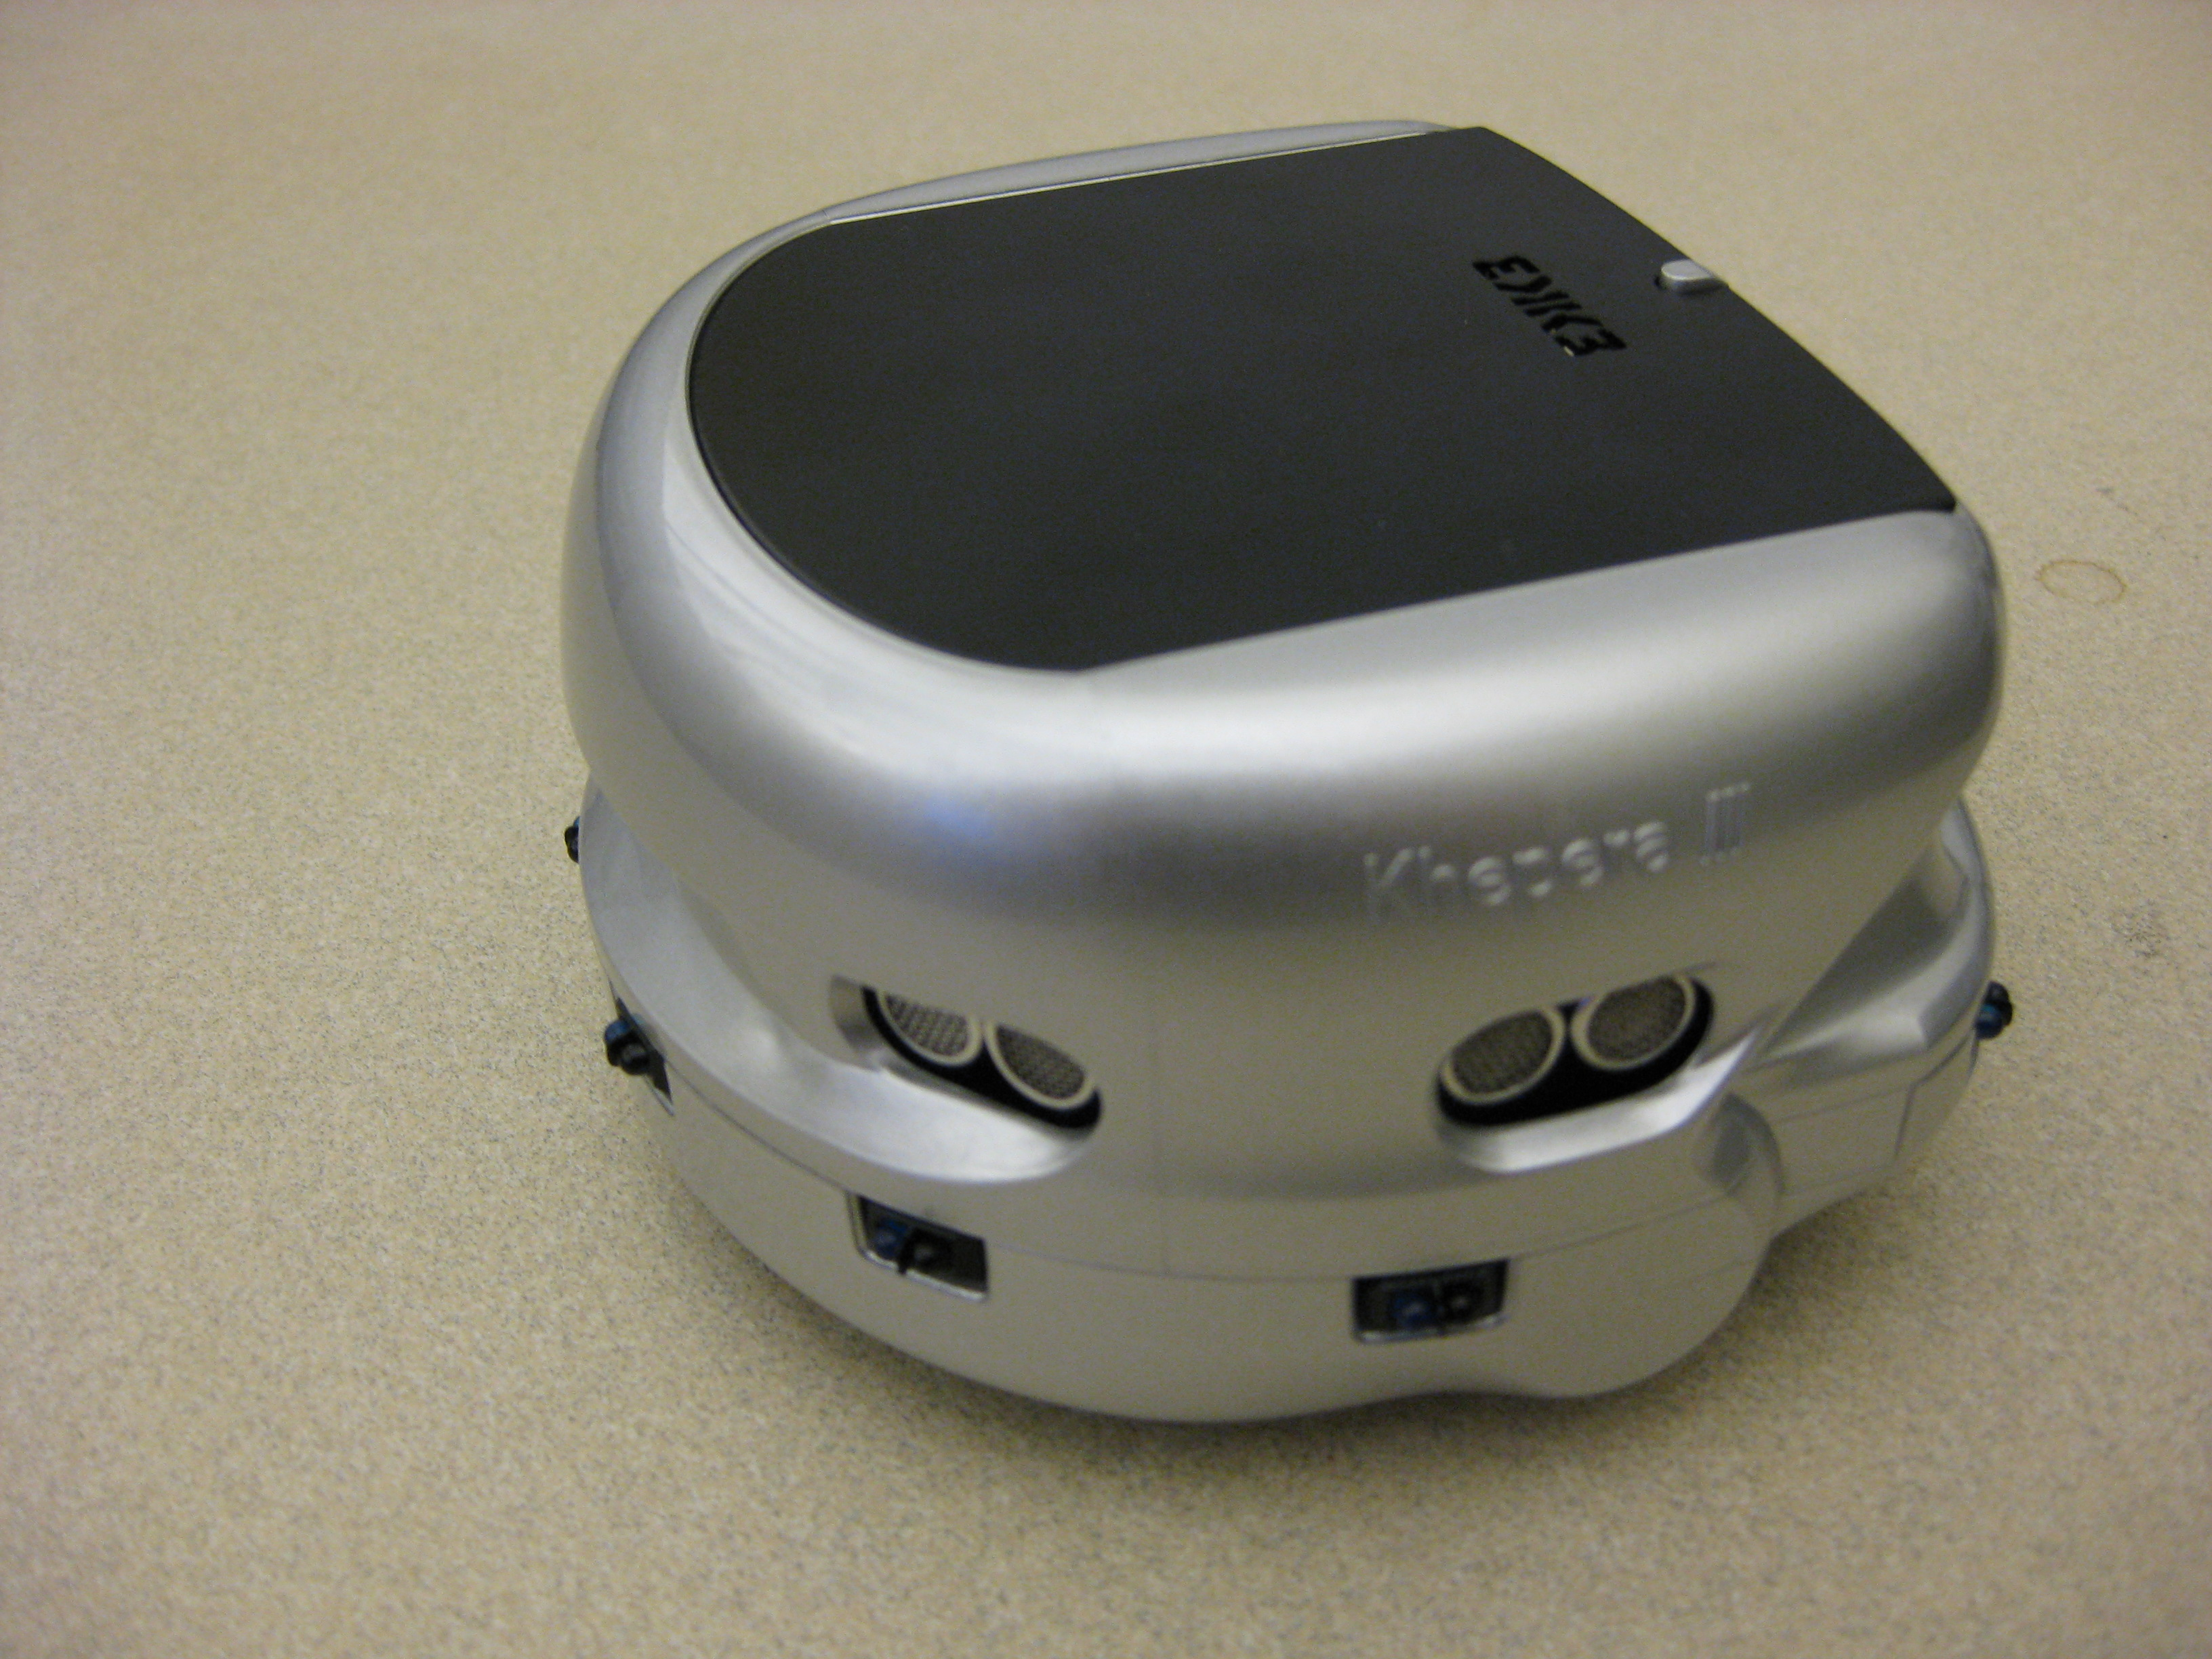
\includegraphics[width=5cm,height=4.5cm]{Figuras/Khepera_III_robot}
%  \subcaption{Robô Khepera}
%  \label{fig:test2}\par\vfill
%  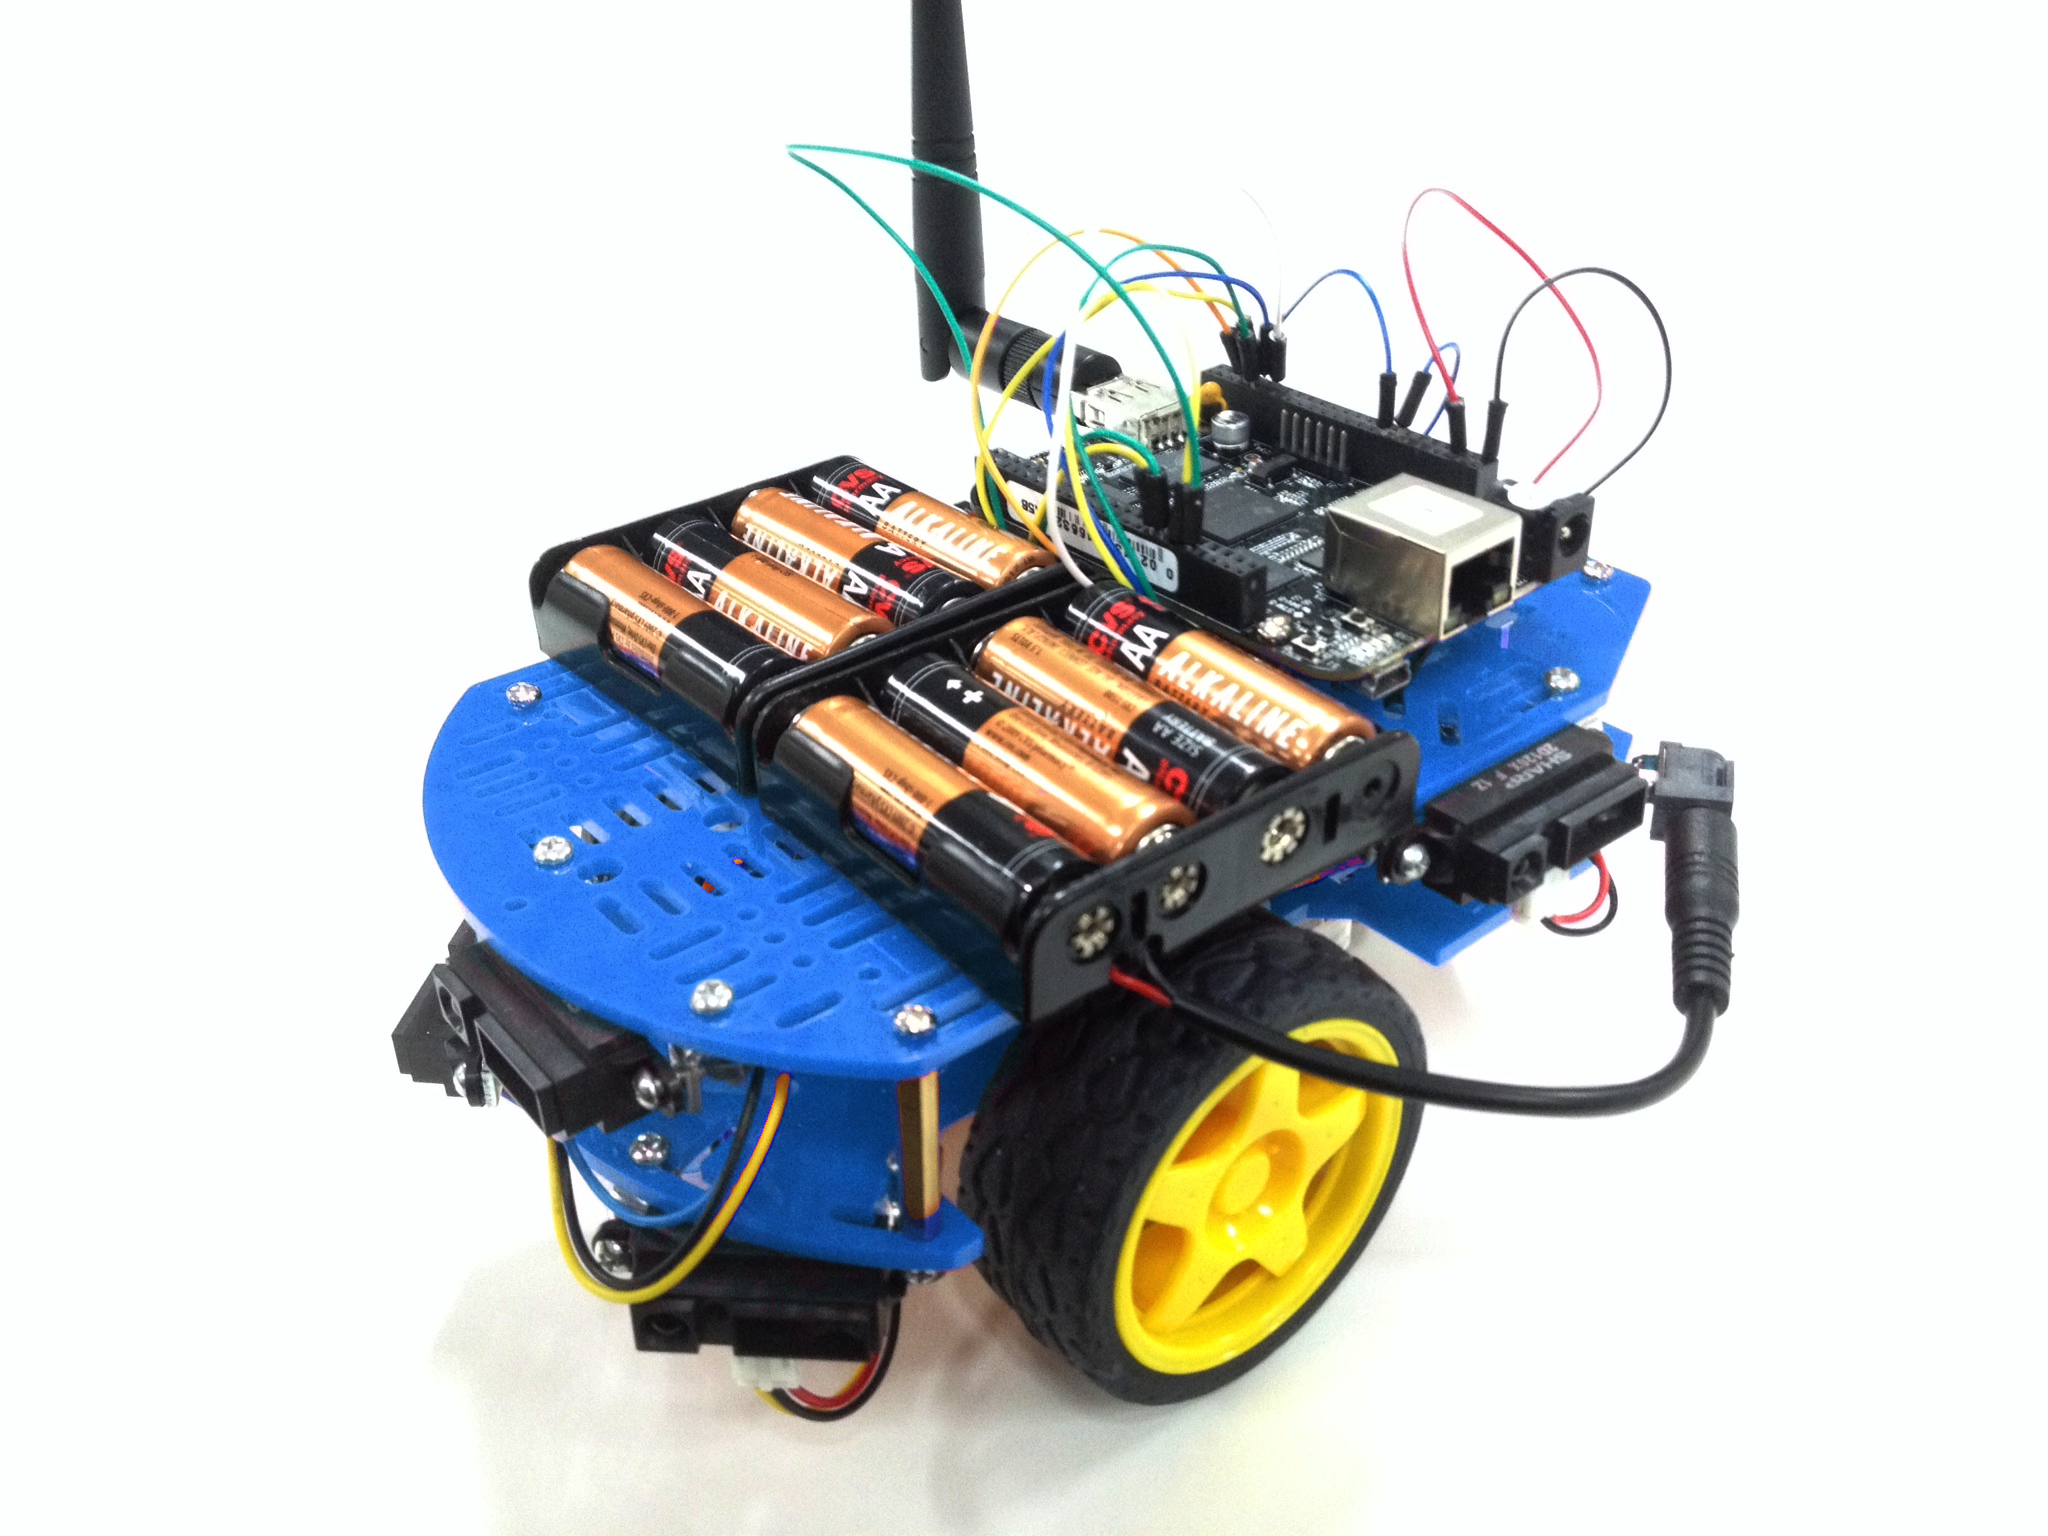
\includegraphics[width=5cm,height=4.5cm]{Figuras/quickbot-blue}
%  \subcaption{Robô QuickBot}
%  \label{fig:test3}
%\end{minipage}
%\begin{minipage}[c][11cm][t]{.5\textwidth}
%  \vspace*{\fill}
%  \centering
%  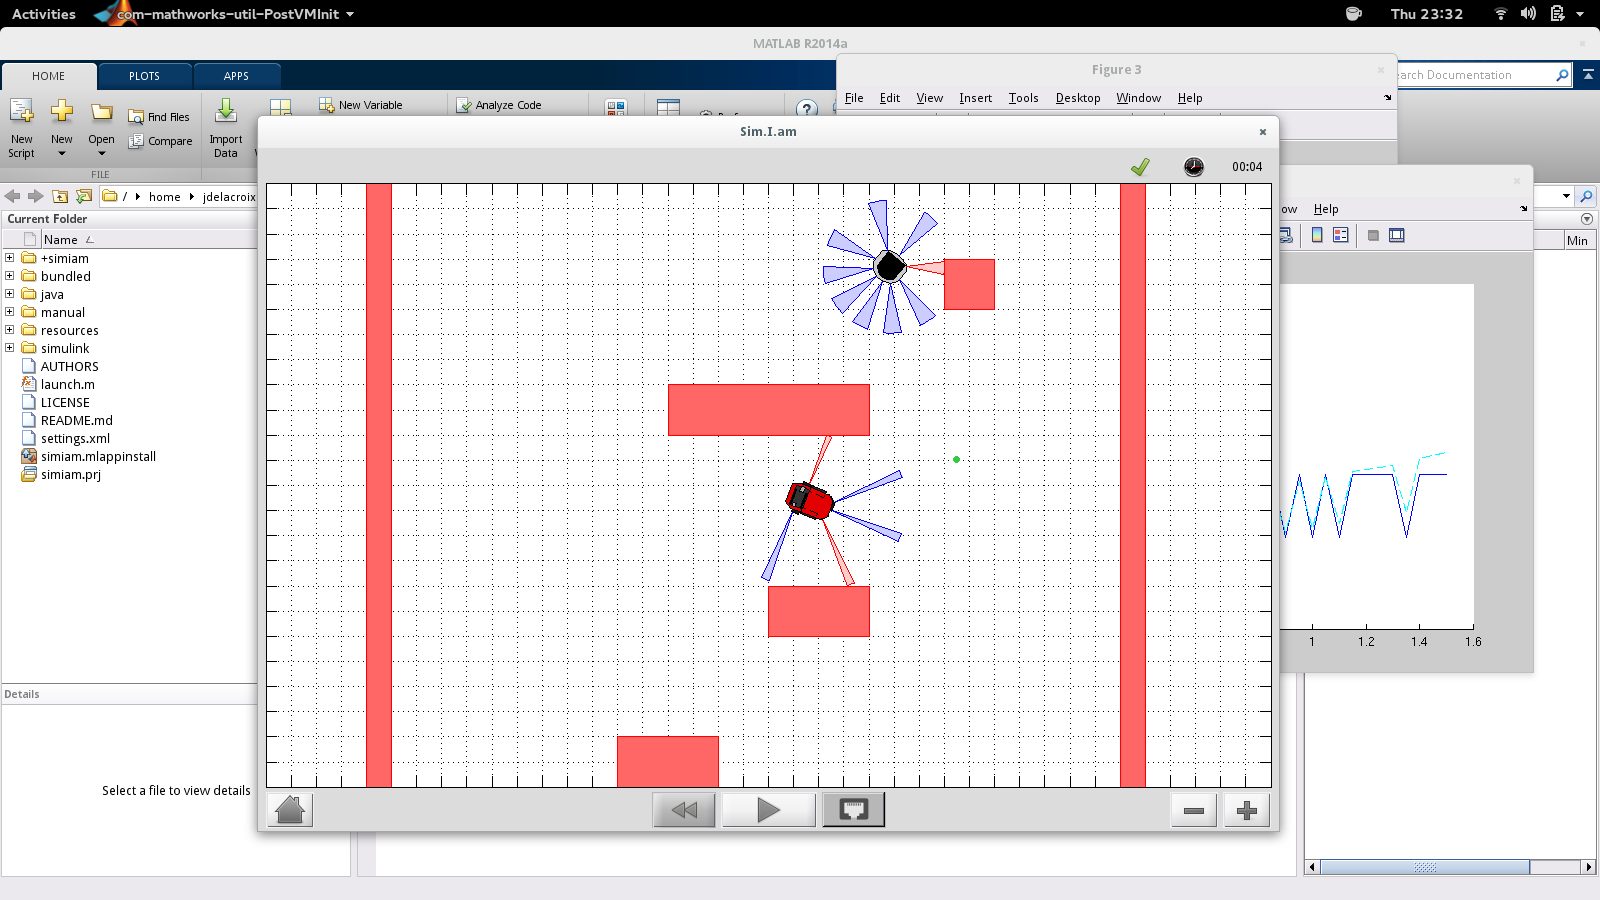
\includegraphics[width=5cm,height=10cm]{Figuras/simiam-screenshot}
%  \subcaption{Simulador Simiam}
%  \label{fig:test1}
%\end{minipage}%
%\end{figure}

\begin{figure}[ht]
\centering
\caption{Robôs Khepera 3 e QuickBot em simulação}
\label{fig:RobosEmSimulador}
		\centering
		% fbox{}
		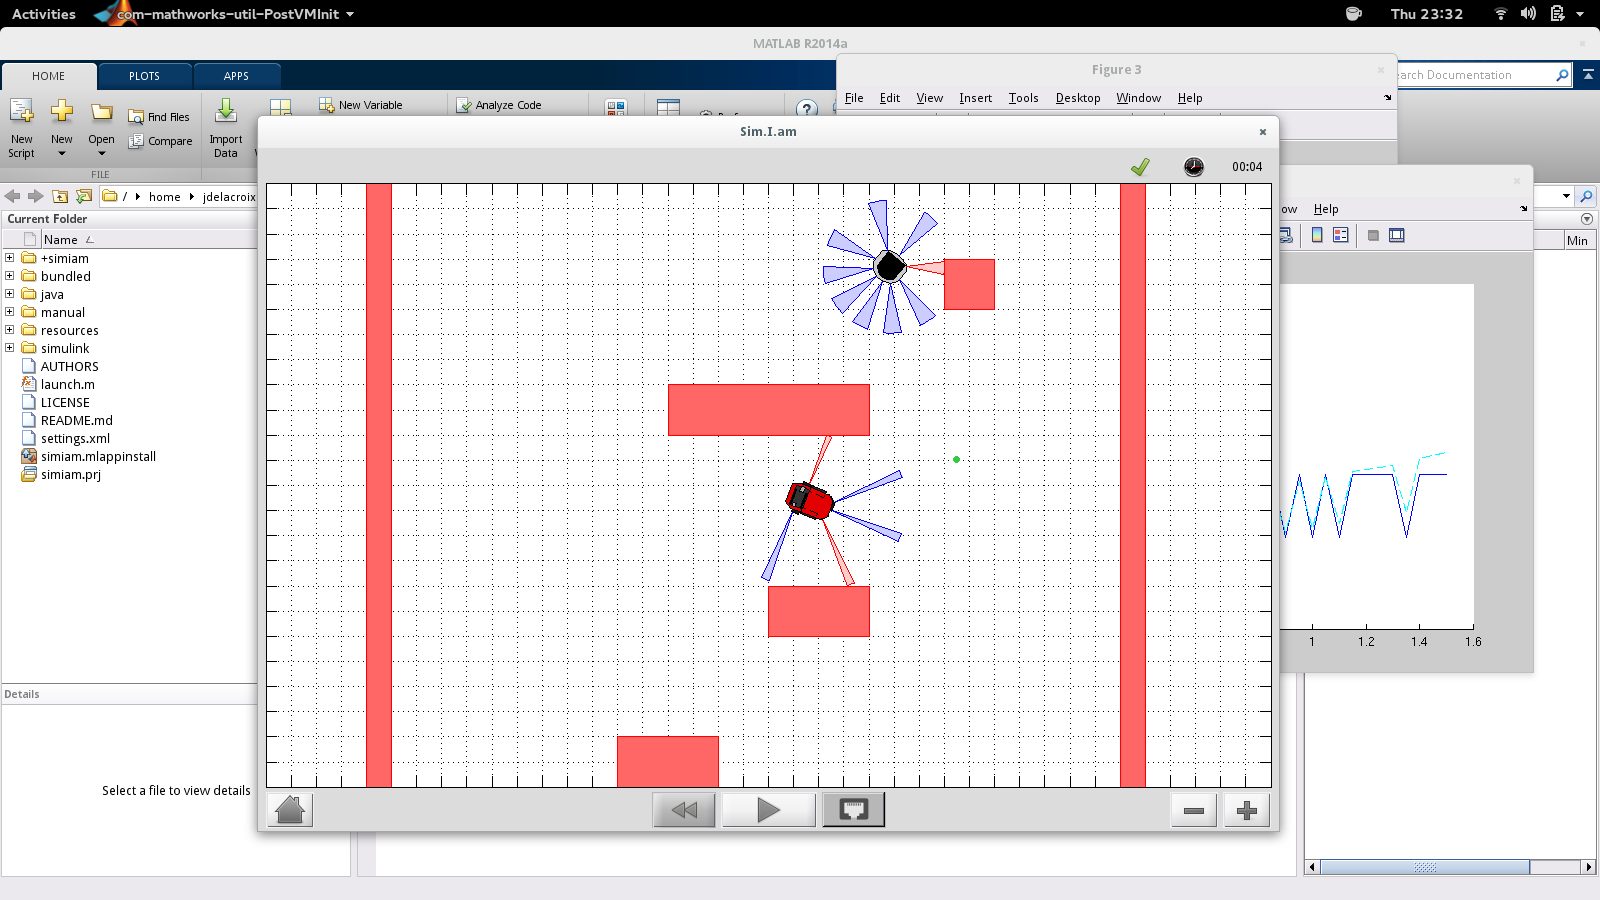
\includegraphics[trim={0cm 0cm 0cm 0cm},clip,
scale=0.24]{Figuras/simiam-screenshot}
	
	\textbf{Fonte: \citeonline{im:Simiam}}
\end{figure}

O Simiam é implementado como um aplicativo Matlab. Possui uma interface
gráfica intuitiva e uma arquitetura interna simples, facilmente customizável. As
subseções a seguir apresentam os pacotes mais importantes, bem como as
principais classes que os compõem e chama atenção para as alterações necessárias
a fim de tornar a simulação coerente com o presente trabalho.

	\subsection{Pacote ``ui''}
	
	O pacote ``ui'' é responsável pela interface gráfica do simulador. A classe
	``AppWindow'' possui um método construtor que inicializa atributos e o
	método ``load\_ui'' que invoca o método ``create\_layout", responsável por
	criar o leiaute da interface.
	
	O botão start, criado pelo método anterior é tratado por ``ui\_button\_start".
	Esta é a função principal reponsável por criar o ambiente de simulação
	(definido no arquivo ``settings.xml''), inserir um ou mais robôs e iniciar a
	simulação.
	
	Alterações mínimas foram efetuadas nesta etapa. Foram adicionados comandos para
	maximizar a janela do simulador e para ajustar o ``zoom'' de modo a permitir uma
	visão panorâmica de todo o ambiente de simulação. O arquivo de configuração
	``settings.xml'' foi alterado a fim de ajustar o ``tamanho do mundo'' ao
	tamanho da	tela.
	
	\subsection{Pacote ``simulator''}
	
	O pacote ``simulator'' realiza de fato a simulação. A classe ``World'' é
	responsável por extrair informações do arquivo ``.xml'', como quantidade e
	localização inicial de robôs e obstáculos, armazenado em estruturas de dados.
	A classe ``Simulator'' atualiza a simulação na janela, enquanto a
	classe ``Physics'' é responsável por detectar colisões de robôs com obstáculos
	e entre si. 
	
	As alterações neste pacote foram todas na classe ``Simulator'', no intuito
	de possibilitar a captura da simulação em video ``.mp4" ou ``.gif". Apesar de
	não ser uma alteração fundamental para a etapa de execução do trabalho, é
	necessária para a apresentação. Não foi criado um botão na interface para
	especificar ao simulador a captura em video. Assim, é necessário, no
	construtor da classe Simulator, atribuir valor verdadeiro aos atributos
	``gravarvideo'' e/ou ``gravargif". 
	
	\subsection{Pacote ``robot''}
	
	O pacote ``robot'' define um ou mais robôs passíveis de serem instanciados. A
	classe ``QuickBot'' estabelece parâmetros físicos, tais como informações
	geométricas, posicionamento dos sensores no corpo do robô e estabelece
	limitações, como velocidades de saturação e zona morta dos motores. Além de
	instanciar objetos das classes ``DifferentialDrive'', ``ProximitySensor'' e
	``WheelEncoder'', ``QuickBot'' extende a classe ``Robot''. 
	
	A classe ``DifferentialDrive" implementa a ``dinâmica'' dos modelos de
	acionamento diferencial e uniciclo. Com os métodos ``uni\_to\_diff'' e ``diff\_to\_uni'', a
	equivalência entre modelo apresentada na Equação \ref{eq:vw_to_diff} é
	estabelecida no espaço de simulação. 

	A classe ``ProximitySensor'' estabelece características do sensor infravermelho
	usado no QuickBot, tais como distâncias mínimas e máximas, espalhamento, localização e
	direção em relação ao corpo do robô e adiciona um ruído gaussiano.
	``WheelEncoder'', similarmente, estabelece características do \textit{encoder}.
	
	As alterações nesta etapa foram no intuito de incluir o robô deste trabalho
	no Simiam. O arquivo ``settings.xml'' deve determinar que um objeto (robô) da
	nova classe criada seja instanciado, ao invés do objeto da classe QuickBot.
	
	\subsection{Pacote ``controller''}
	
	O pacote ``controller'' é responsável pela implementação de todos os
	controladores e supervisores dos robôs implementados. A classe ``Supervisor'' é
	extendida para obter o controlador supervisório de cada robô a ser simulado.
	Para o QuickBot e Khepera 3, os respectivos supervisores são definidos pelas
	classes ``QBSupervisor'' e ``K3Supervisor''. Essas classes definem máquinas de
	estado, onde cada estado é associado a um controlador de variável contínua.
	Esses controladores, por sua vez, extendem a classe ``Controller'' e
	implementam os ``comportamentos'', ou modos, dos robôs.
	% Calculo de odometria está em QBSupervisor.
	
	As alterações neste pacote foram responsáveis pela inclusão de suporte a
	controladores \textit{Fuzzy}, além de adicionar o supervisório específico para
	o robô desenvolvido.
	 
\section{Montagem física do robô}

Os componentes físicos do robô podem ser vistos na Figura \ref{fig:RoboReal}.a e
o resultado após montagem está retratado na Figura \ref{fig:RoboReal}.b.

\begin{figure}[!ht]
\centering
\caption{Materiais e robô após montagem}
\label{fig:RoboReal}
	\begin{subfigure}[b]{0.49\textwidth}%
		\centering
		% fbox{}
		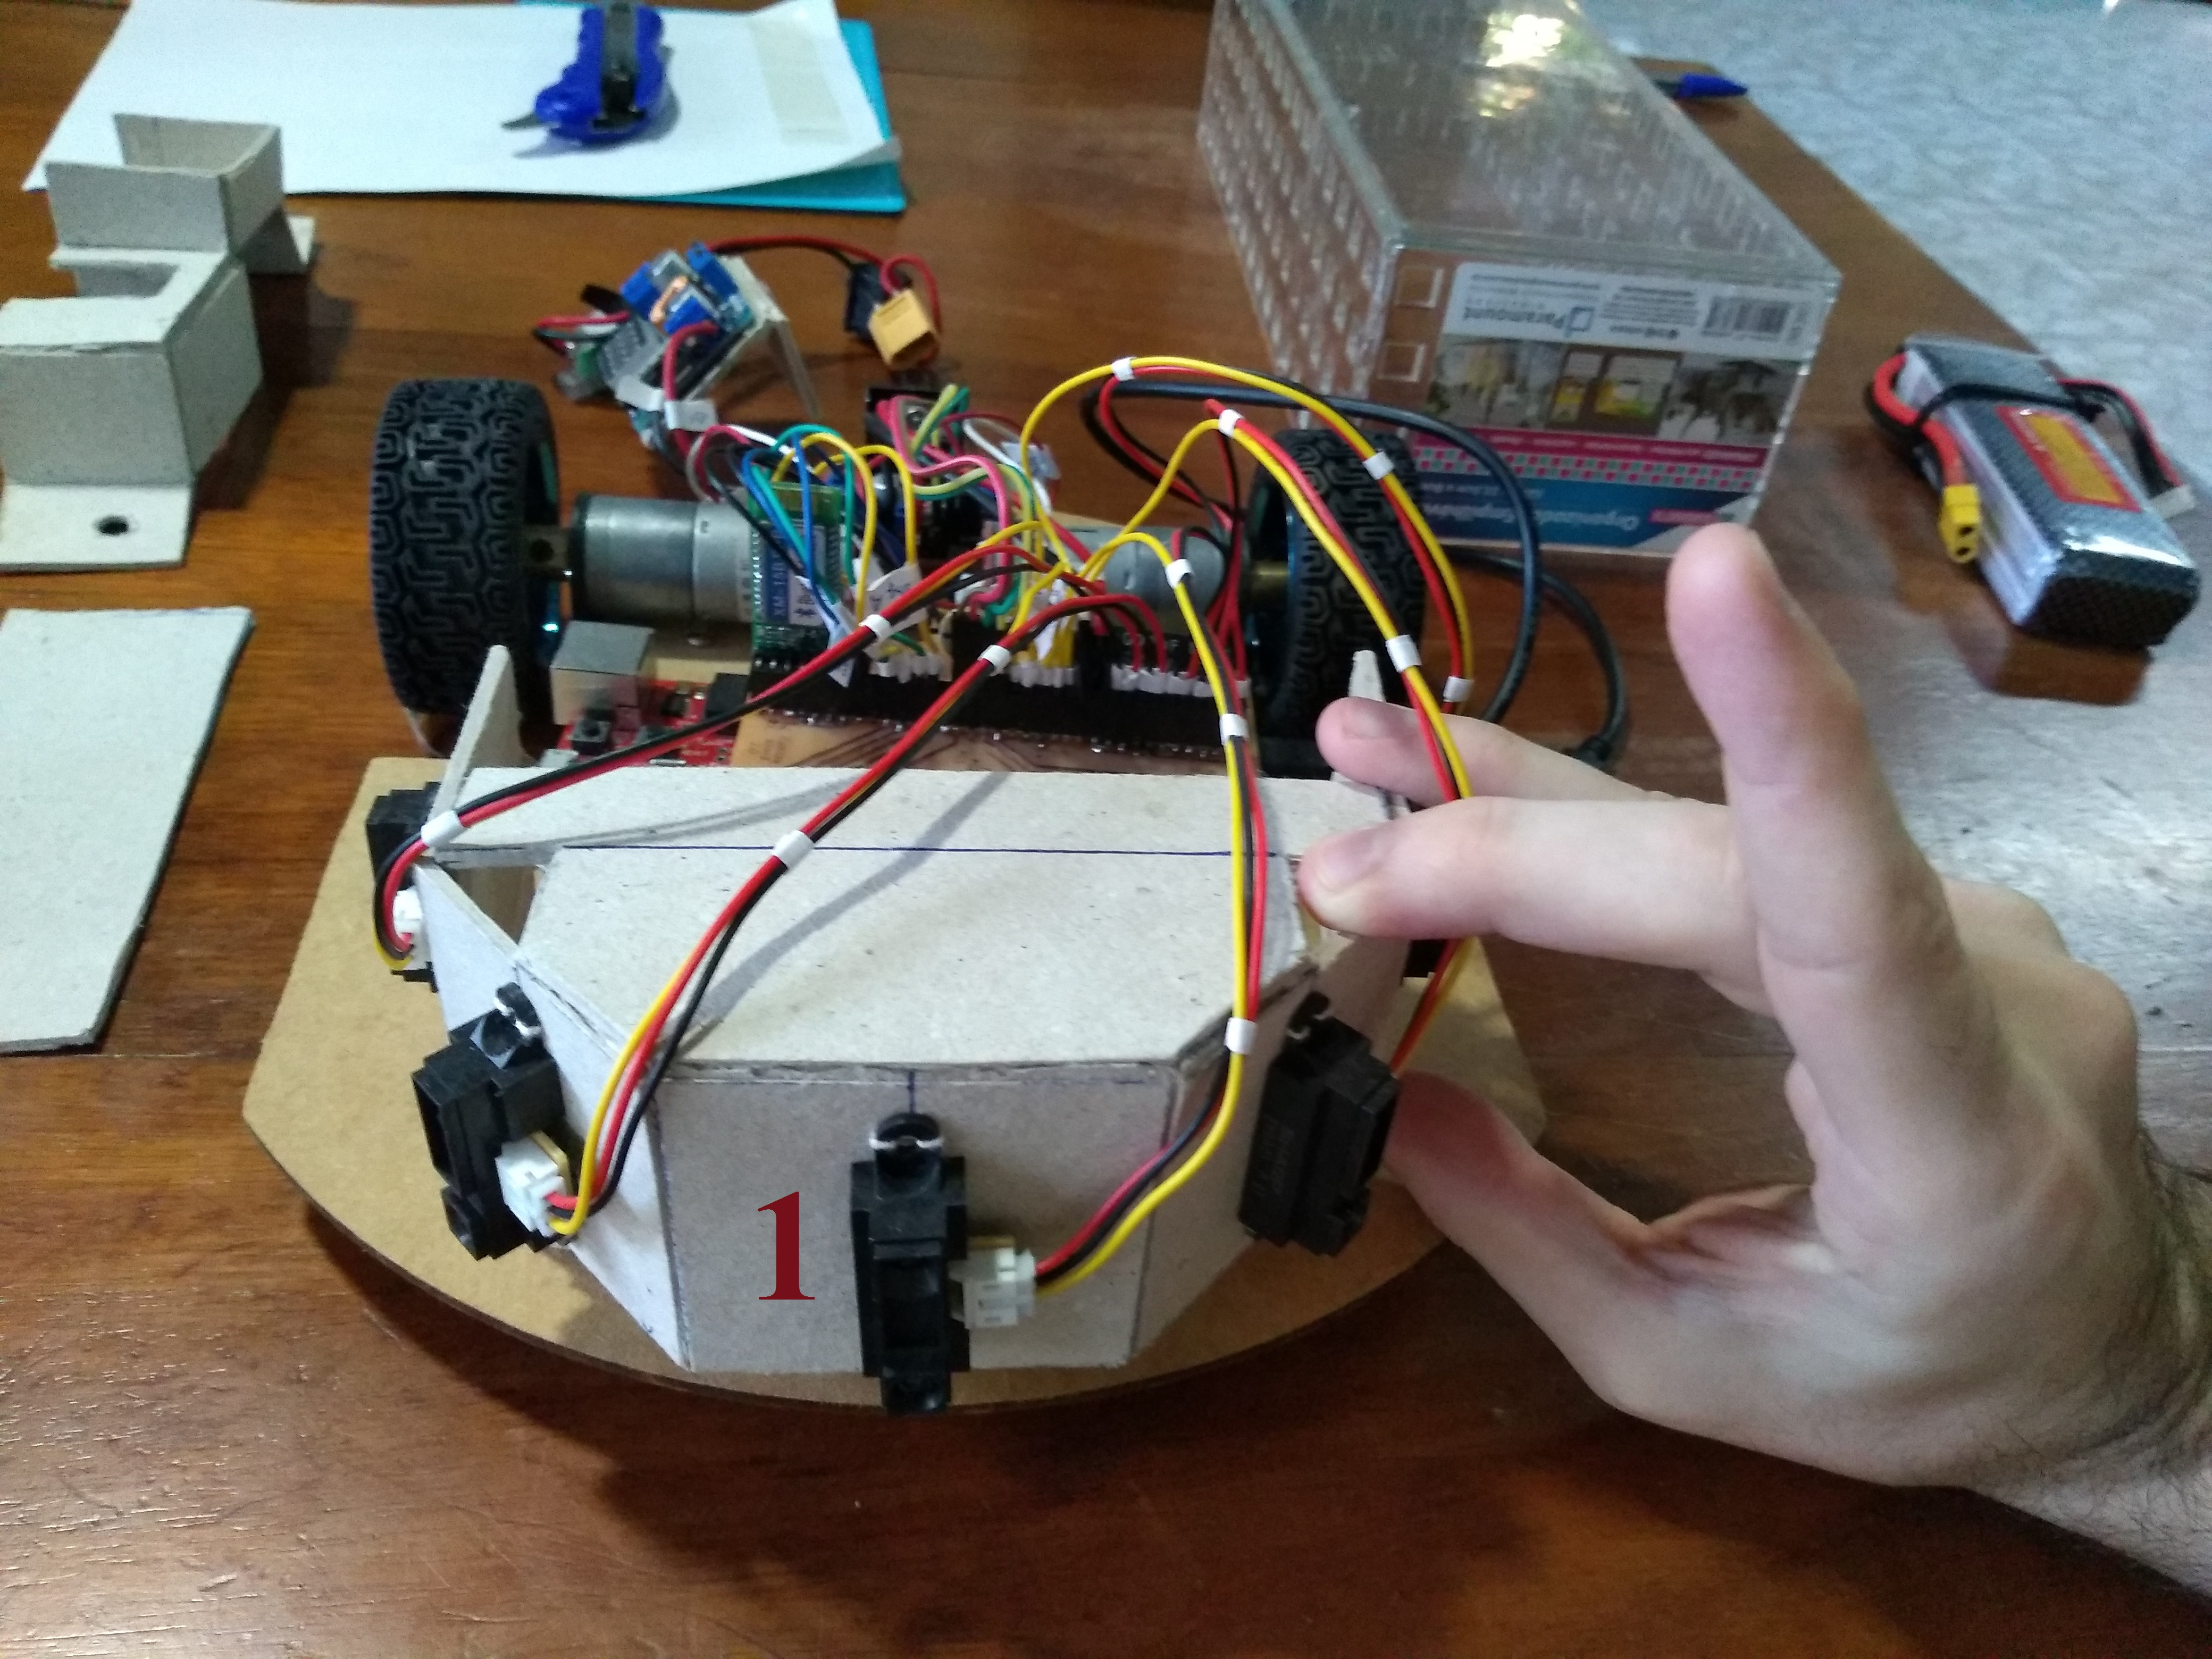
\includegraphics[trim= 0cm 0cm 0cm 0cm,clip,
scale=0.055]{Figuras/RoboMontagem1}
		\subcaption{Posicionamento dos sensores IR}
	  	%\label{fig:test1}
	\end{subfigure}
	~
	\begin{subfigure}[b]{0.49\textwidth}%
		\centering
		% fbox{}
		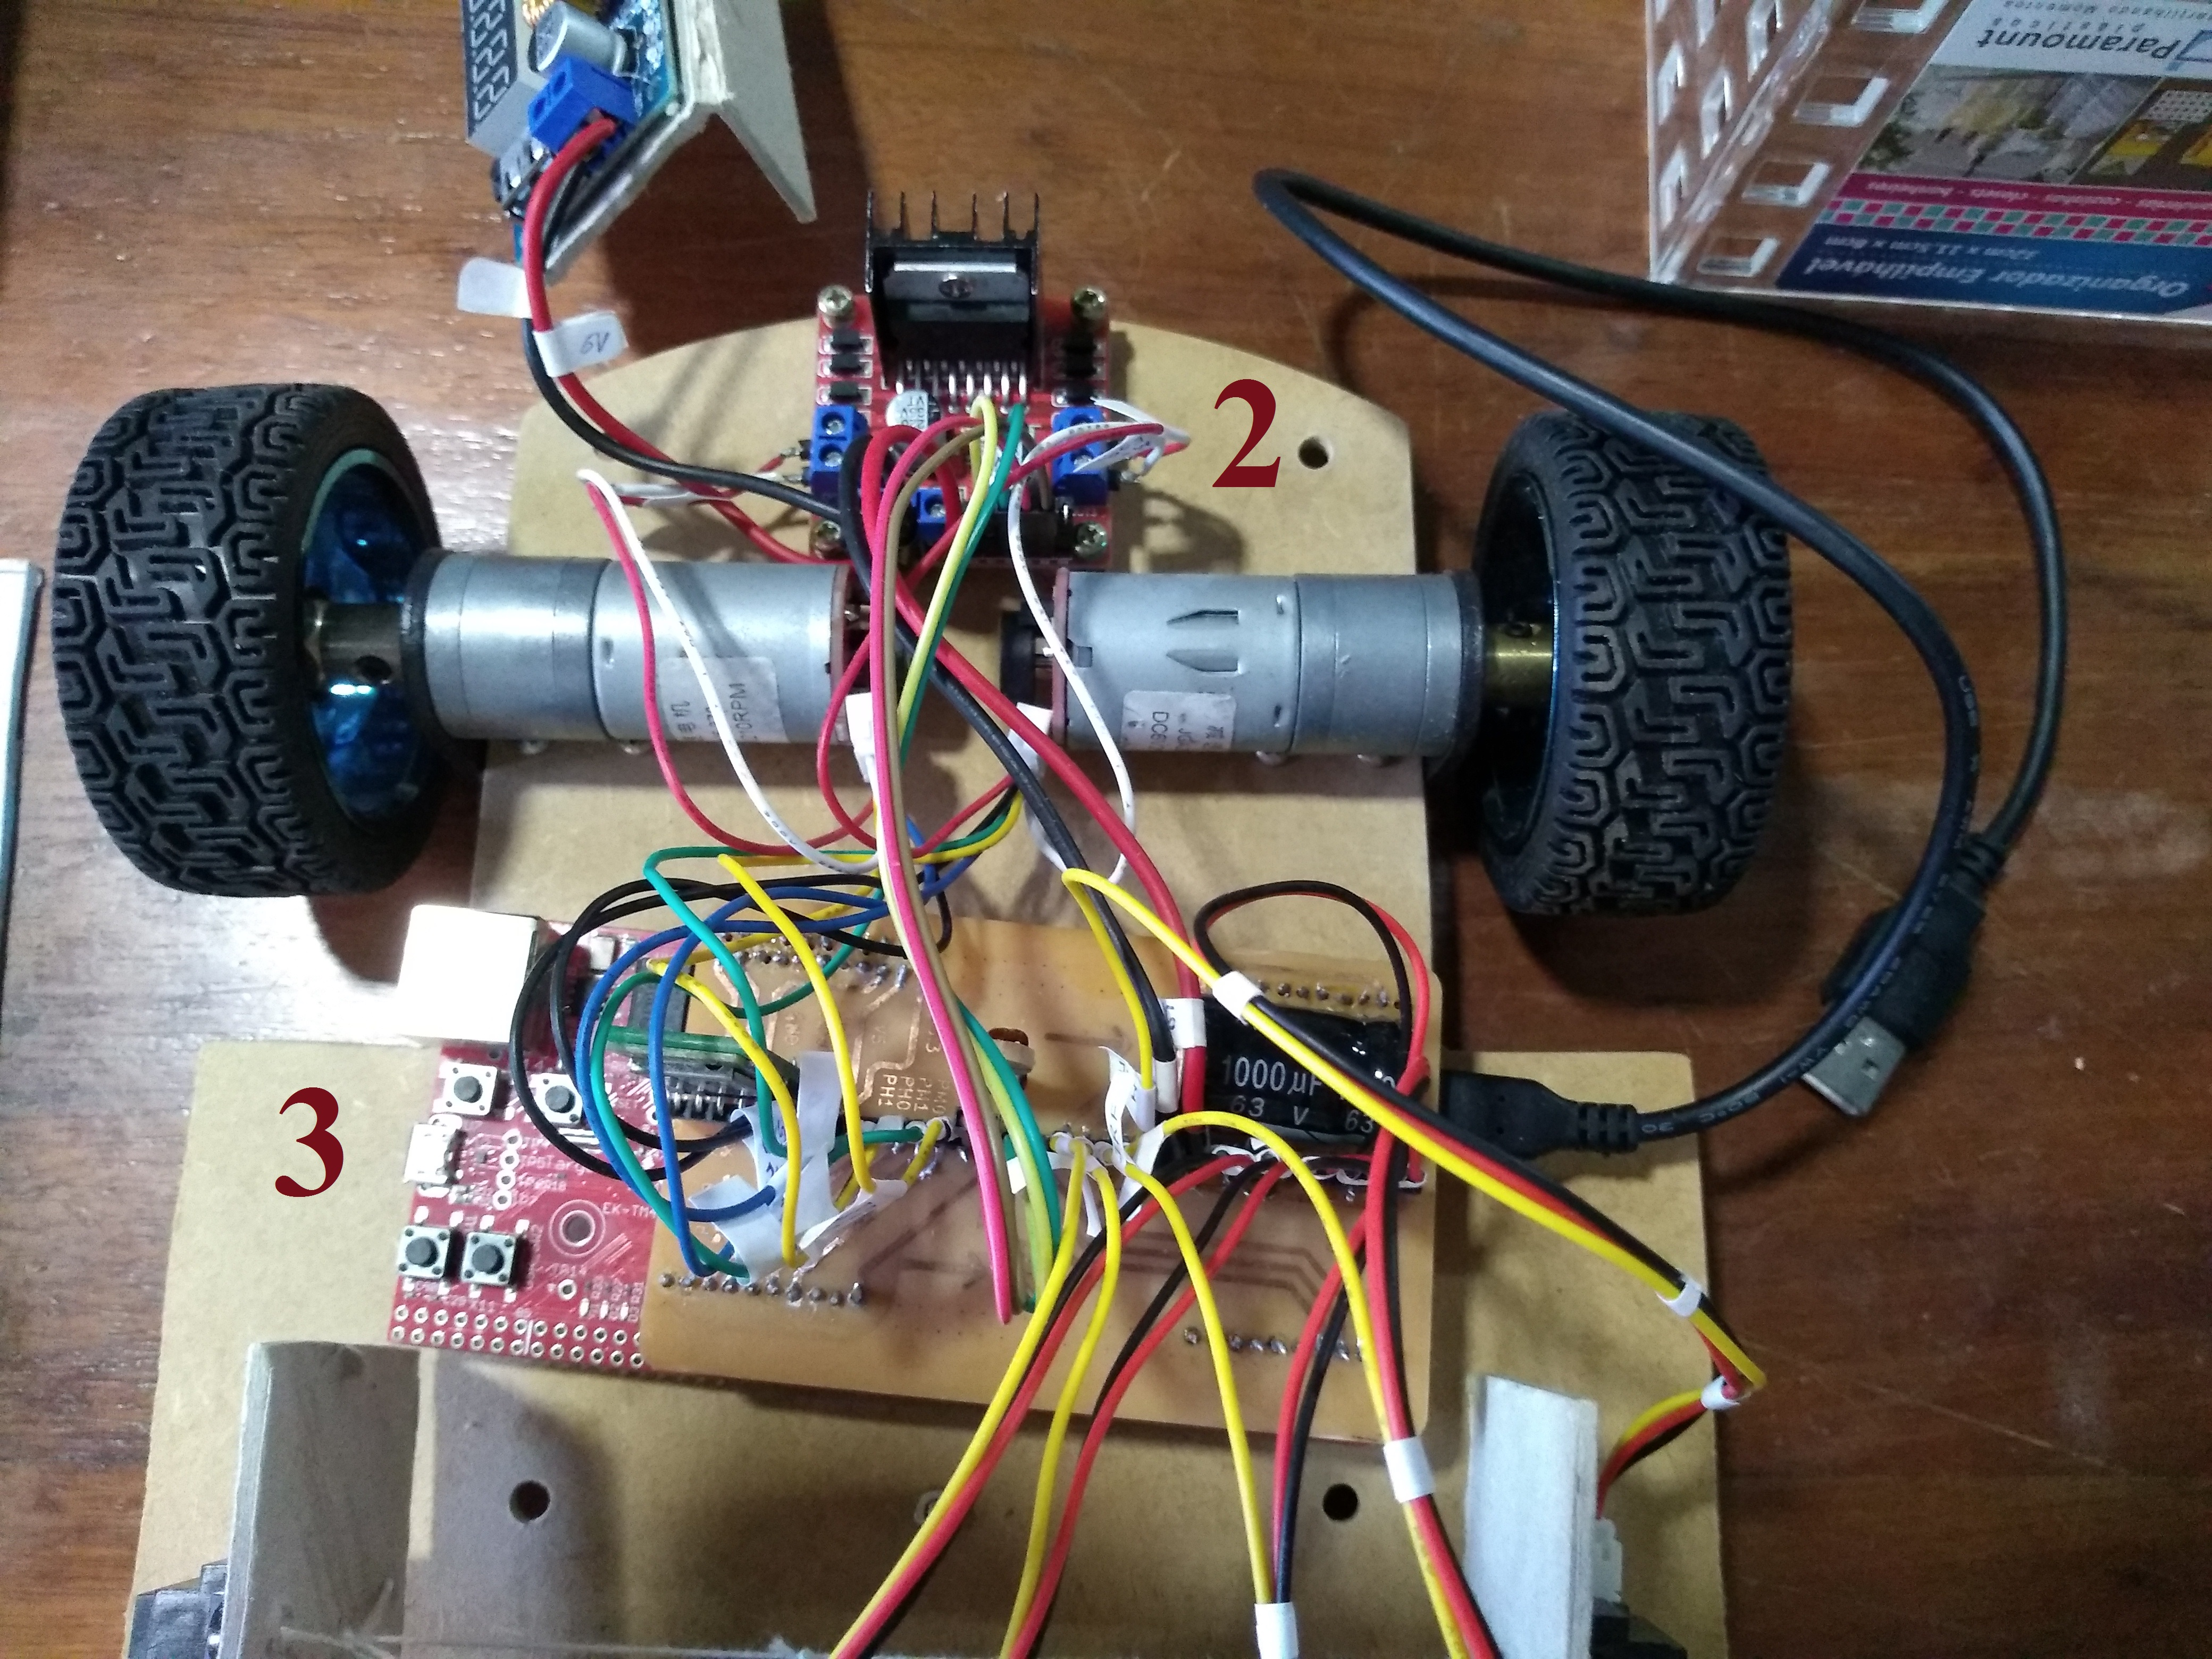
\includegraphics[trim={0cm 0cm 0cm 0cm},clip,
scale=0.055]{Figuras/RoboMontagem2}
		\subcaption{Disposição dos motores e microcontrolador}
	  	%\label{fig:test2}
	\end{subfigure}
	~
	\begin{subfigure}[b]{0.49\textwidth}%
		\centering
		% fbox{}
		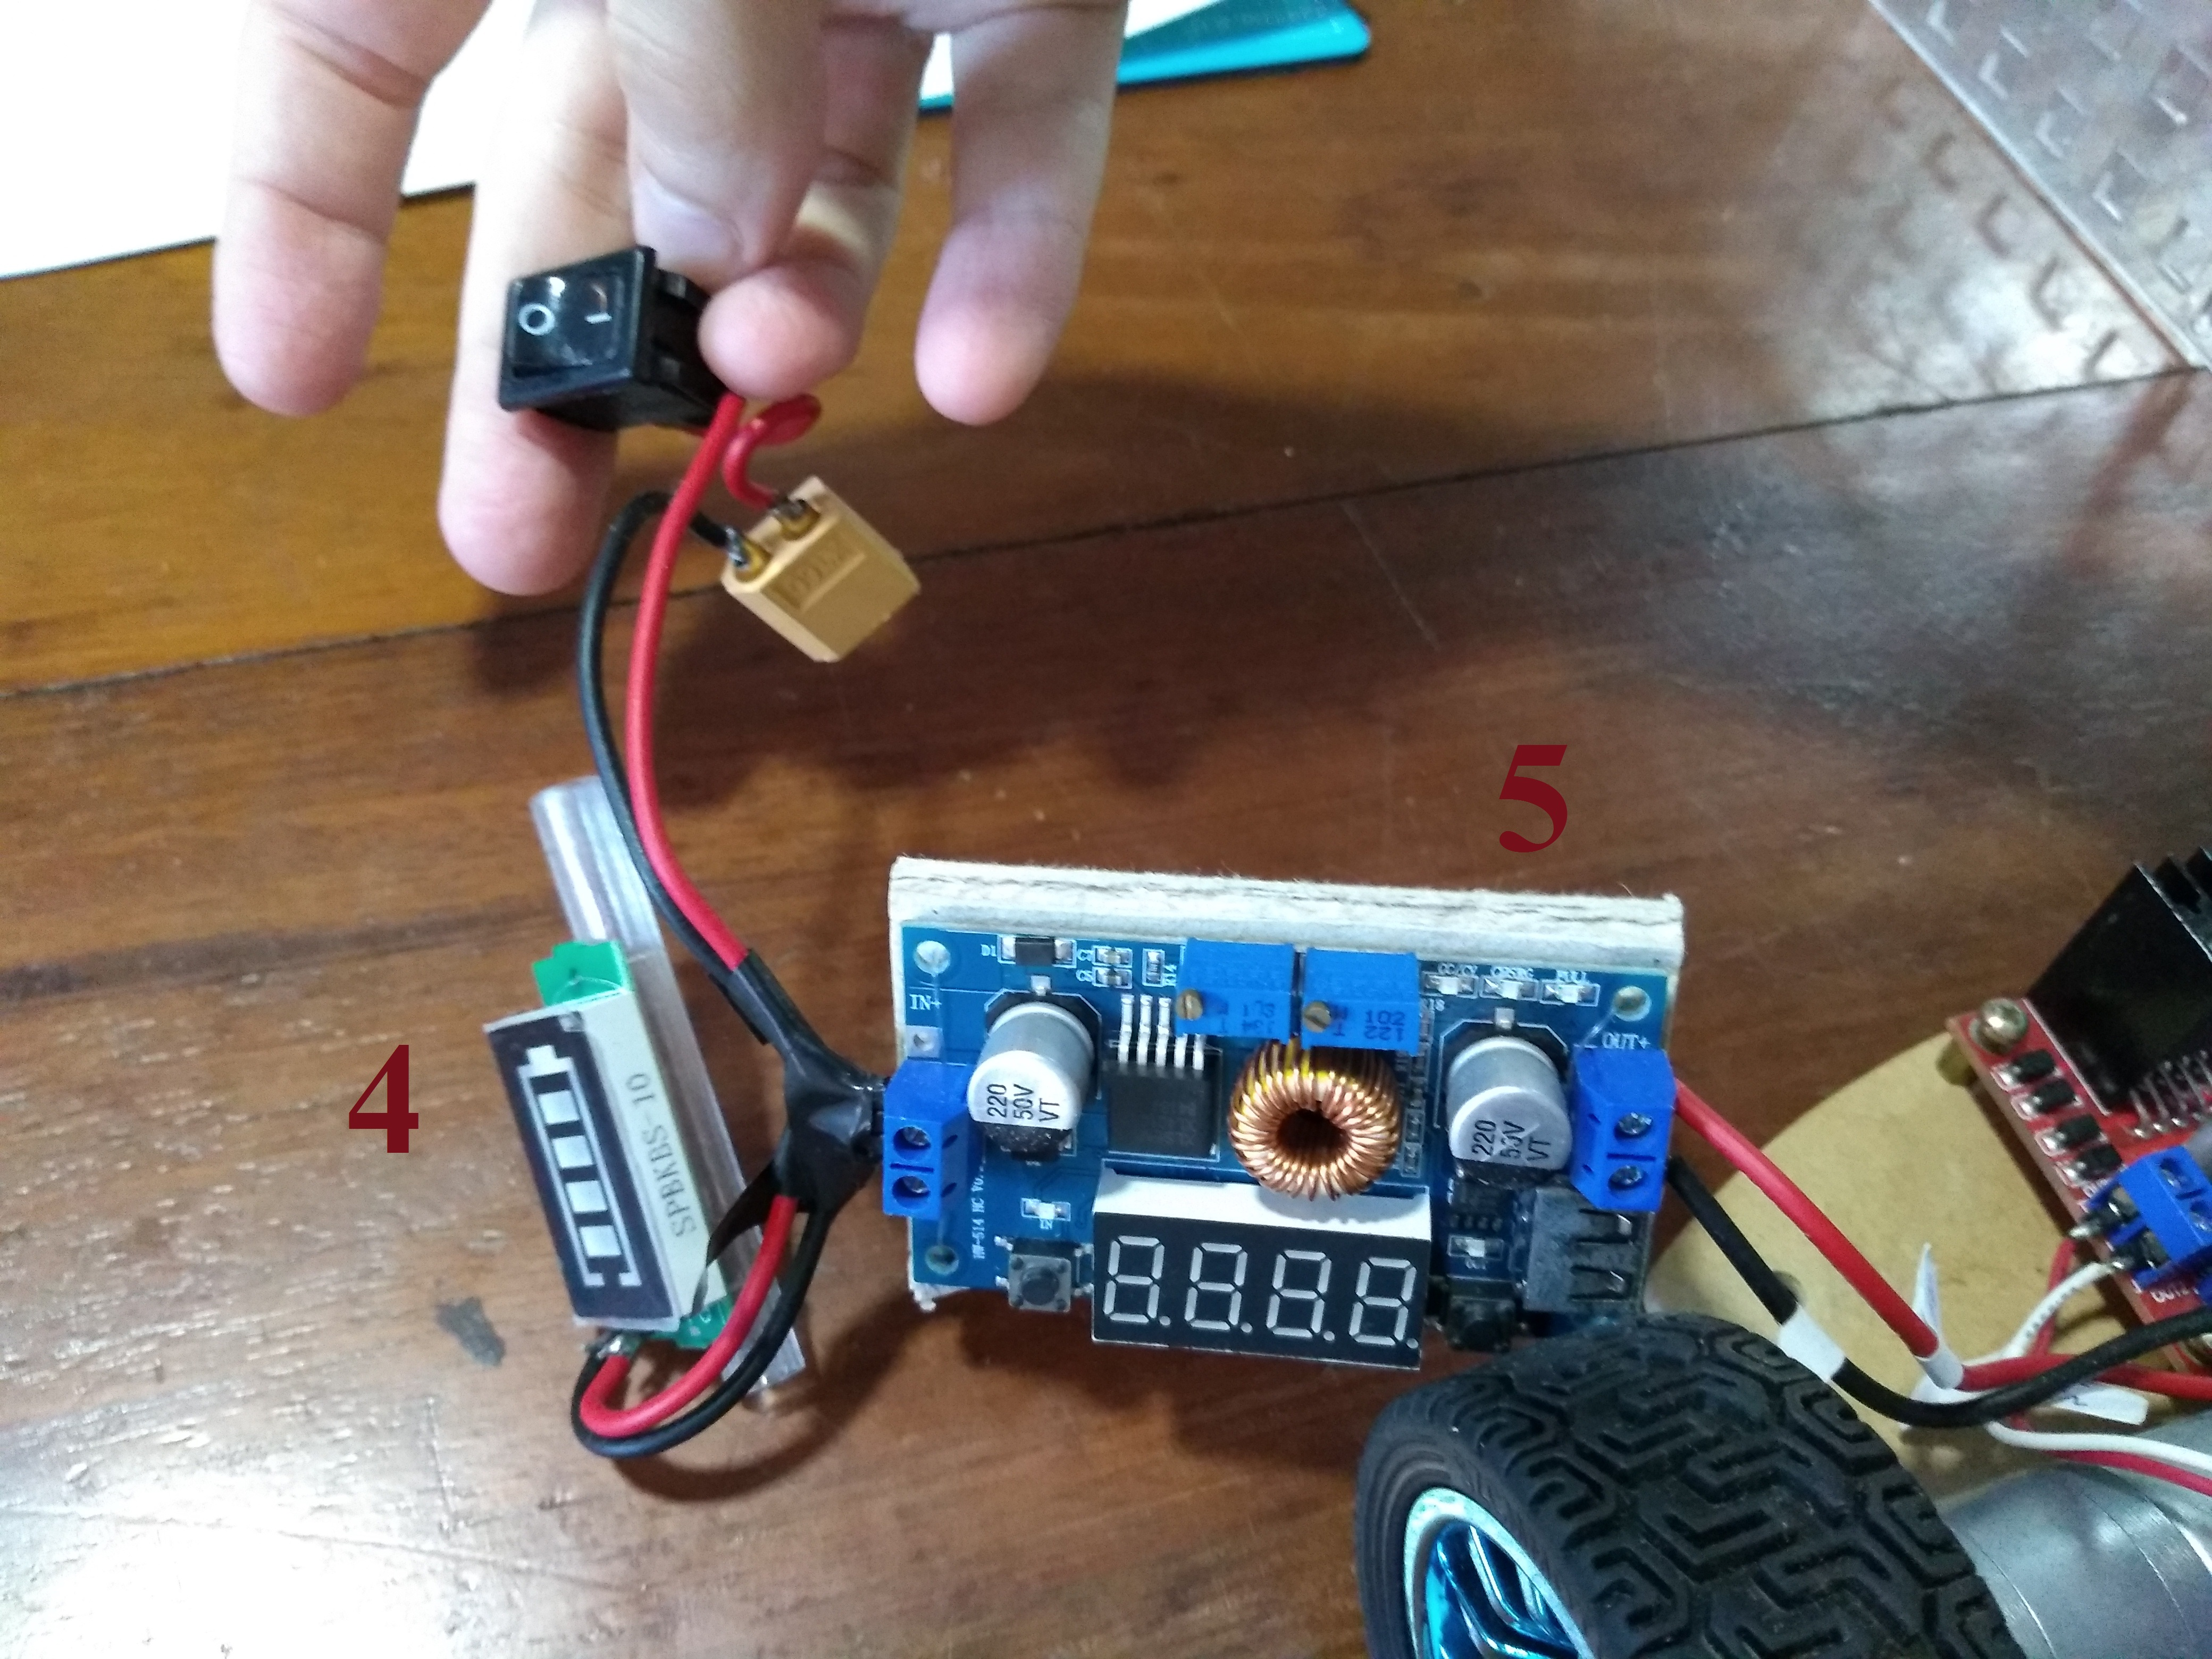
\includegraphics[trim= 0cm 0cm 0cm 0cm,clip,
scale=0.055]{Figuras/RoboMontagem3}
		\subcaption{Regulador de Tensão}
	  	%\label{fig:test1}
	\end{subfigure}
	~
	\begin{subfigure}[b]{0.49\textwidth}%
		\centering
		% fbox{}
		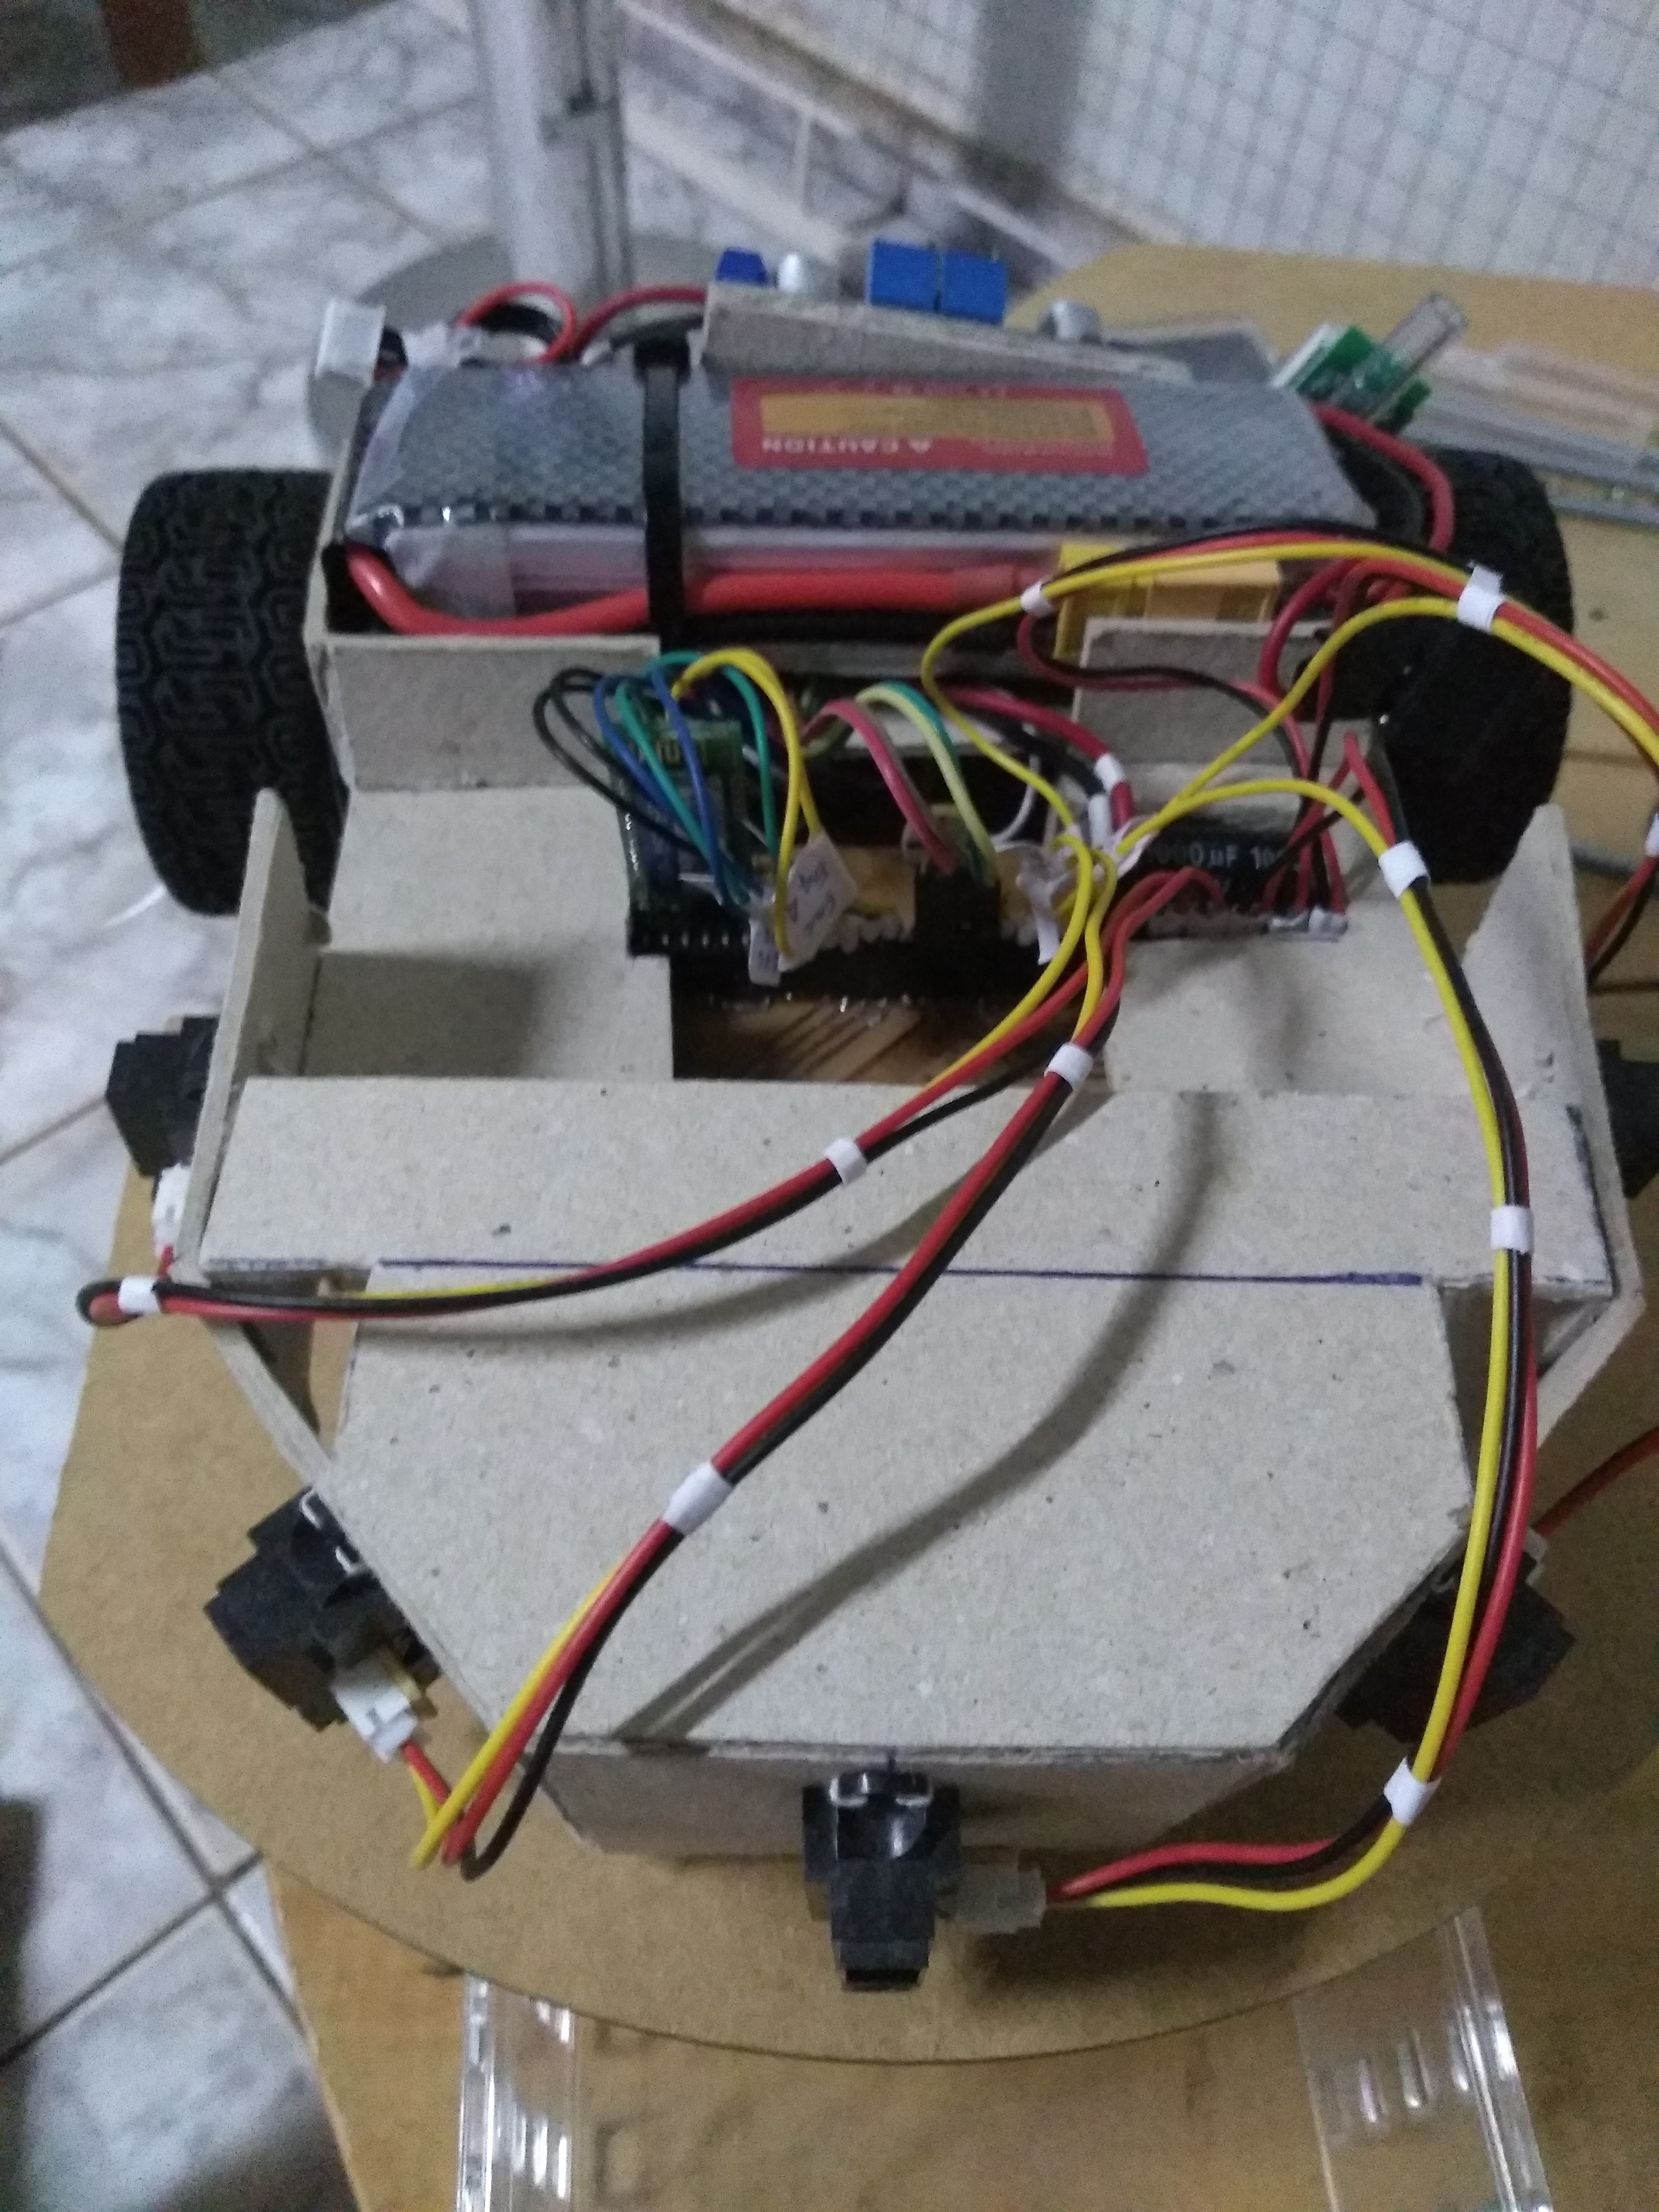
\includegraphics[trim={0cm 0cm 0cm 0cm},clip,
scale=0.055]{Figuras/RoboMontagem4}
		\subcaption{Posicionamento dos componentes}
	  	%\label{fig:test2}
	\end{subfigure}
	
	\textbf{Fonte: autoria própria}
\end{figure}

\subsection{Especificações}

As variáveis L e R na Equação \ref{eq:diff}, para o robô deste trabalho, valem
respectivamente 18 cm e 3,4 cm.

O sensor infravermelho GP2Y0A21YK0F utilizado neste trabalho possui a curva de
tensão por distância representada na Figura \ref{fig:SensorIR}. A faixa de
distância está entre 10 e 80 cm. No QuickBot, é utilizado o sensor GP2Y0A41SK0F,
com distância de medição entre 4 e 30 cm.

\begin{figure}[ht]
	\centering
	\caption{Resposta do sensor infravermelho}
	\label{fig:SensorIR}
	
	%\fbox{}
	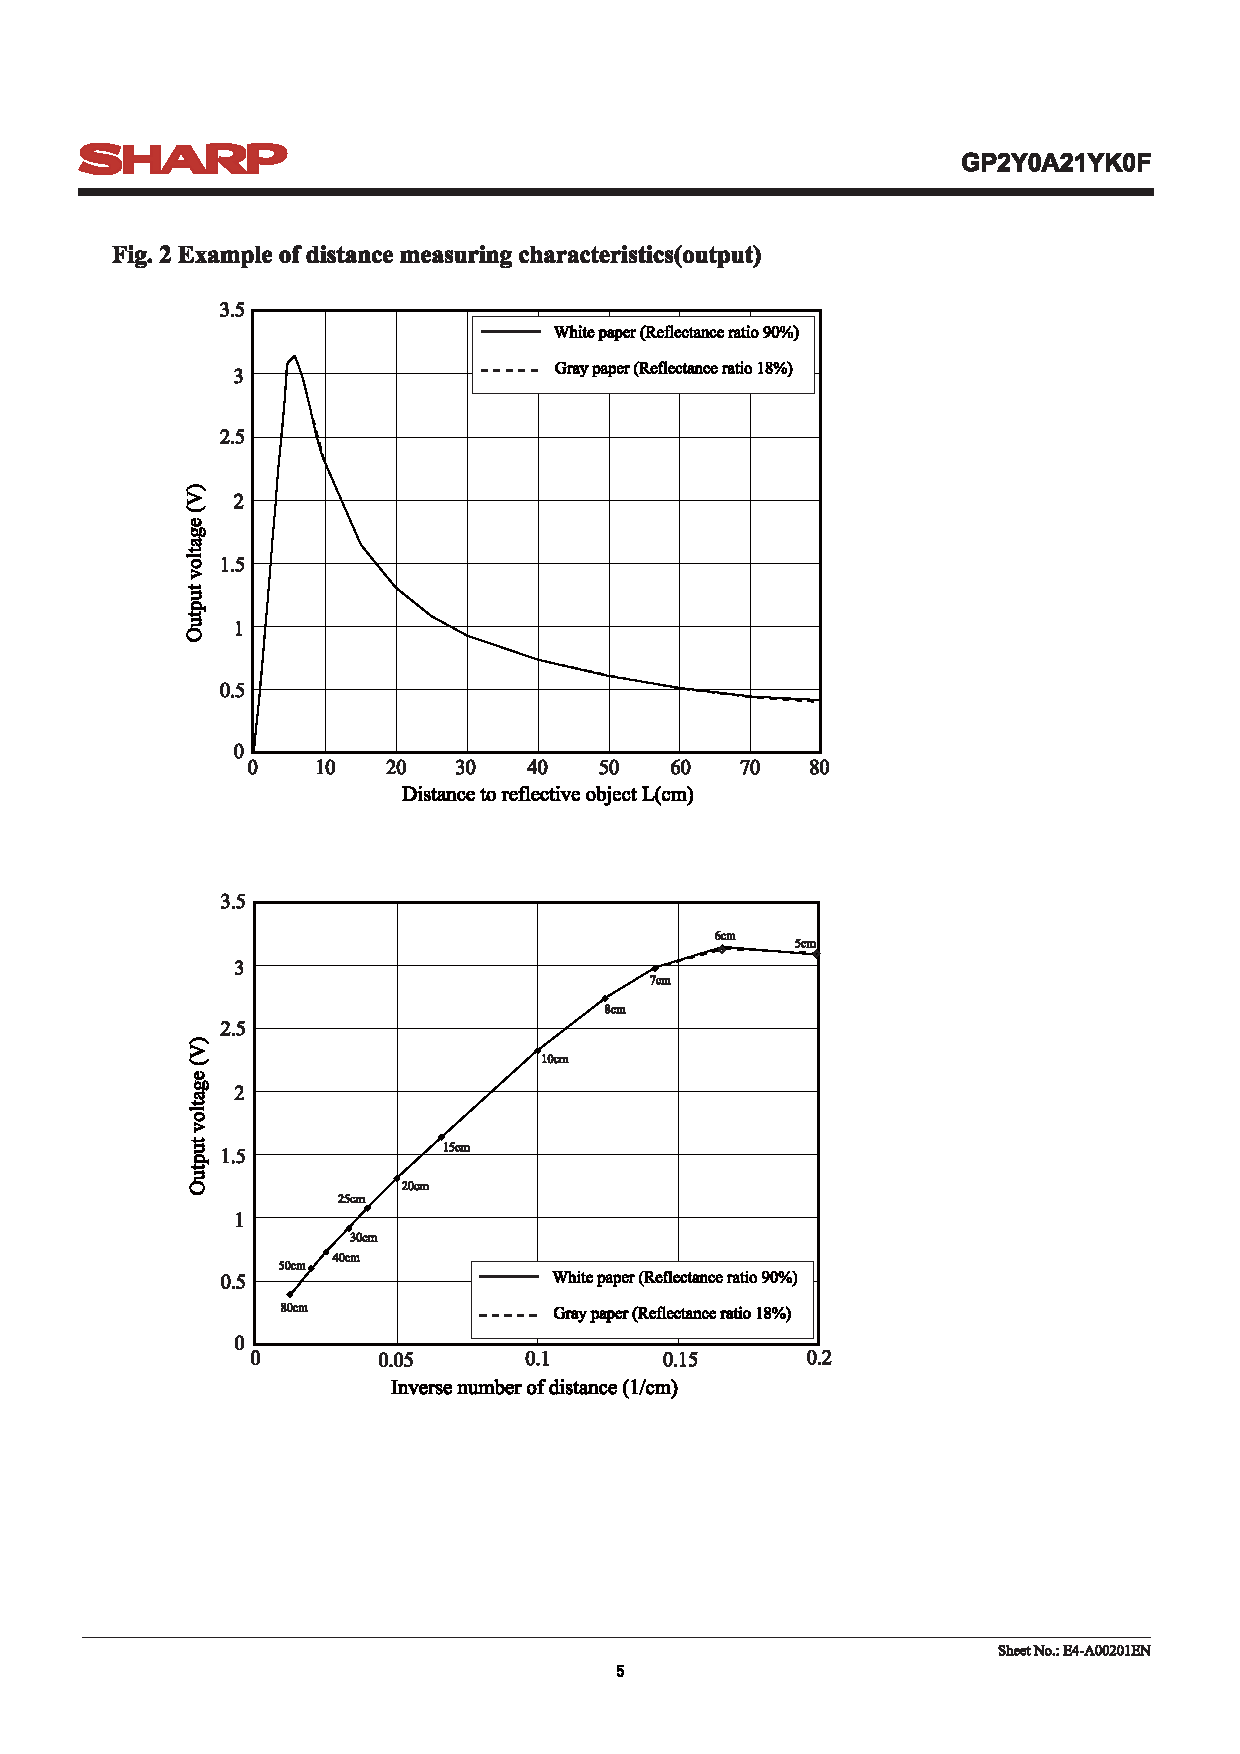
\includegraphics[trim= 3cm 15.8cm 6.5cm 4.8cm,clip,
scale=1]{Figuras/IR_Datasheet_Figure}

	%\begin{tikzpicture}[auto, node distance=2cm, on grid,
%>=latex']%
	
	%\node[anchor=south west,inner sep=0] (image) at (0,0) {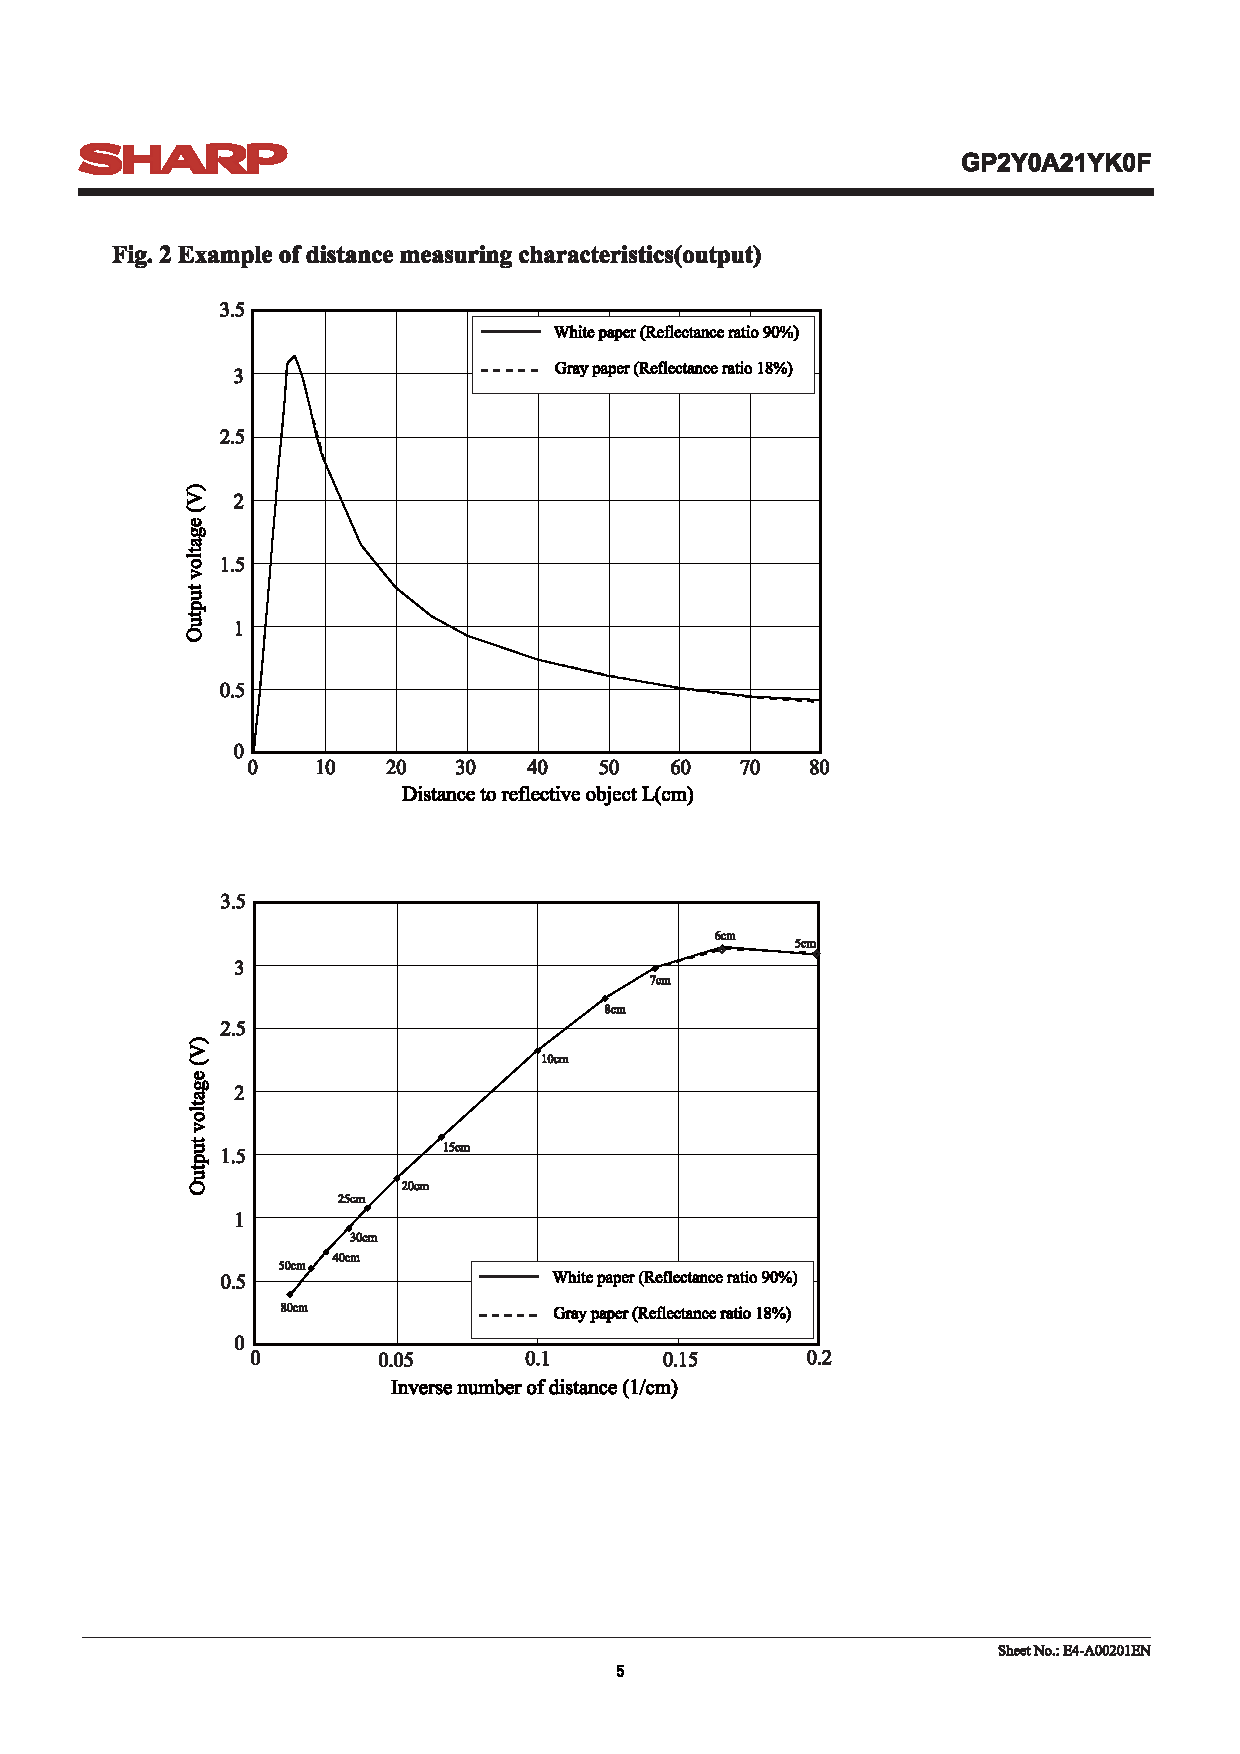
\includegraphics[trim =
%		{3cm 15.8cm 6.5cm 4.8cm}, clip,scale=1]{Figuras/IR_Datasheet_Figure}};
		
%	\node[fill,circle,inner sep=0.1pt, color = red] at (1.29,1.161) {};
%	\node[fill,circle,inner sep=0.1pt, color = red] at (2.525,2.235) {};
	
%	\node[fill,circle,inner sep=0.1pt, color = red] at (1.83,7.75) {};
	
	
%	\node[inner sep = 0 pt, outer sep = 0 pt] (origin) at (1.3,1.15) {};
%	\node[inner sep = 0 pt, outer sep = 0 pt] (teste2) at (2.55,2.25) {};
%	
%	\node[inner sep = 0 pt, outer sep = 0 pt] (P1) at (1.85,7.85) {};
	
	%\draw[-, color = red] (origin) -- (teste2);
	%\draw[-, color = red] (origin) -- (P1);
	
	%\node[] at (0,0) {};
	%\coordinate[] (teste1) {};
	%\coordinate[] (teste2) {};
	
	%\draw[-, color = red] (-18,2) -- (-7,3);
	
%	\end{tikzpicture}


	\textbf{Fonte: \citeonline{datasheet:SensorIR}}
\end{figure}

Para a região da curva onde $d > 5,5 cm$, o polinômio que a aproxima, associando
o inverso da distância pela tensão ($d(v) = \frac{1}{d'(v)}$), obtido utilizando
a função polyfit do Matlab pode ser visto na Equação \ref{eq:PolinomioVx}.
\begin{equation}
	\label{eq:PolinomioVx}
	d'(v) = 21.49298 v^5 + 21.86894 v^4 + 22.25754 v^3 + 22.65912 v^2 + 23.07406 v
	+ 23.50272
\end{equation}

%Odometria

\section{Desenvolvimento dos controladores}

	Nesta seção pretende-se investigar a arquitetura comportamental em robótica 
	móvel para as duas estratégias clássicas de implementação: arbitragem e fusão de 
	comportamentos. Para isso, controladores híbrido e fuzzy serão criados, o primeiro
	para arbitrágem e o segundo para fusão.

	\subsection{Por Controlador Híbrido}
	
	Nesta subseção, pretende-se demonstrar um controlador simples capaz de 
	solucionar o problema de navegação, usando autômato híbrido. Para cada estado
	no autômato, um controlador é selecionado e uma recomendação de saída é 
	calculada. 
	
		\subsubsection{Comportamento ''Ir Para Objetivo''}
		
		\newcommand{\meuRoboLindaoCompIPO}{
	\begin{tikzpicture}[scale = 2]%
		\coordsystwo{I}
		\begin{scope}[shift={(3, 0.9)}]
			\draw[->] (0.3,0) arc (0:30:0.3);
			\draw[-] (0,0) -- (0.4,0);
			\node at (0.5,0.1) {$\phi$};
			
			% Pr 
			\begin{scope}[scale = 0.5]
				\node[color = gray] at (0.1,-0.35) {$P_r$};
			\end{scope}
			\begin{scope}[rotate=30,scale=0.5]
				\begin{scope}[scale=0.9]
					\coordsystwo{R}
				\end{scope}
				\begin{scope}[shift={(0.25,0)},rotate = -90]
					\RoboDiffClean
				\end{scope}
			\end{scope}	
		\end{scope}
		
		% Coord objetivo
		\begin{scope}[shift={(4, 3)}]
			\filldraw (0,0) circle (1pt);
			% Po
			\begin{scope}[scale = 0.5]
				\node[color = gray] at (0.2,-0.45) {$P_o$};
			\end{scope}
		\end{scope}
		
		% retas
		\node[inner sep = 3pt] (P1) at (4,3) {};
		\node[inner sep = 3pt] (P2) at (3,0.9) {};
		
		\draw[->] (0,0) -- (P1);
		\draw[->] (0,0) -- (P2);
		\draw[->] (P2) -- (P1);
		
		% angulo do objetivo
		\draw[->] (0.6,0) arc (0:37:0.6);
		\draw[-] (0,0) -- (0.4,0);
		\node at (0.8,0.4) {$\theta$};
	\end{tikzpicture}%
}%

\newcommand{\RoboDiffClean}{
	% Linhas de baixo, lat esq e dir
	\draw[-, inner sep = 0] (-0.65,-0.75) -- (0.65,-0.75);
	\draw[-, inner sep = 0] (-0.75,-0.65) -- (-0.75,0.5);
	\draw[-, inner sep = 0] (0.75,-0.65) -- (0.75,0.5);
	
	% bordas de baixo
	\draw[-, inner sep = 0] (-0.65,-0.75) -- (-0.75,-0.65);
	\draw[-, inner sep = 0] (0.65,-0.75) -- (0.75,-0.65);
	
	% Retas de cima
	\def\UserL{\fpeval{1.3/(2*cosd(45)+1)}}
	\draw[-, inner sep = 0] (-0.75,0.5) -- (\fpeval{-0.75+\UserL*cosd(45)},
	\fpeval{0.5+\UserL*sind(45)});
	
	\draw[-, inner sep = 0] (0.75,0.5) -- (\fpeval{0.75-\UserL*cosd(45)},
	\fpeval{0.5+\UserL*sind(45)});
	
	\draw[-, inner sep = 0]
	(\fpeval{-0.75+\UserL*cosd(45)},\fpeval{0.5+\UserL*sind(45)}) -- (\fpeval{0.75-\UserL*cosd(45)},
	\fpeval{0.5+\UserL*sind(45)});
	
	% Bola de rolamento
	\filldraw (0,0.45) circle (1.5pt);
	\draw (0,0.45) circle (3pt);
	
	% Desenhar rodas
	\begin{scope}[shift={(-0.75,-0.65)},rotate = 90]
		\draw[rounded corners=2pt] (0,0) rectangle ++(0.8,0.2);
	\end{scope}
	\begin{scope}[shift={(0.75,-0.65)},rotate = 90]
		\draw[rounded corners=2pt] (0,0) rectangle ++(0.8,-0.2);
	\end{scope}	
}

\begin{figure}[ht]
	\centering%
	\caption{Comportamento Ir para Objetivo}%
	\label{fig:CompIPO}%	
	\meuRoboLindaoCompIPO
	
	\textbf{Fonte: autoria própria}
\end{figure}
		
		\subsubsection{Comportamento ''Evitar Obstáculo''}
		
		\newcommand{\meuRoboLindaoCompEO}{

	\begin{scope}[shift={(0,0.3)}]
		% Pr 
		\begin{scope}[shift={(0,-0.3)}, scale = 0.5]
			\node[color = gray] at (0.1,-0.35) {$P_r$};
		\end{scope}
		\begin{scope}[rotate=90,scale=0.5]
			\filldraw (0,0) circle (0.5pt);
			\begin{scope}[shift={(0.25,0)},rotate = -90]
				\RoboDiffClean
			\end{scope}
		\end{scope}
	\end{scope}
		
	% Obstáculo
	\begin{scope}[shift={(2,0)}]
		\obstaculo{3}
	\end{scope}
}%

\newcommand{\obstaculo}[1]{
	\node[inner sep = 0pt] (P1) at (0,0) {};
	\node[inner sep = 0pt] (P2) at (0.5,0) {};
	\node[inner sep = 0pt] (P3) at (0.5,#1) {};
	\node[inner sep = 0pt] (P4) at (0,#1) {};
	\draw (P1) -- (P2);
	\draw (P2) -- (P3);
	\draw (P3) -- (P4);
	\draw (P4) -- (P1);
}

\newcommand{\sensorVisaoTriangular}[1]{
	\draw (0,0) -- (-0.1,#1);
	\draw (0,0) -- (0.1,#1);
	\draw (-0.1,#1) -- (0.1,#1);
}

\newcommand{\sensorVisaoVetor}[1]{
	\draw[->] (0,0) -- (0,#1);
}

\newcommand{\desenharSensoresTriangulo}{
	\node[color = gray] at (-2.58,0.6) {$d_1$};
	\node[color = gray] at (-1.82,2.41) {$d_2$};
	\node[color = gray] at (0,3.07) {$d_3$};
	\node[color = gray] at (1.82,2.41) {$d_4$};
	\node[color = gray] at (2.24,0.6) {$d_5$};
	
	\begin{scope}[shift={(0.38,0.6)},rotate=-90]
		\sensorVisaoTriangular{2-0.38}
	\end{scope}
	\begin{scope}[shift={(-0.38,0.6)},rotate=90]
		\sensorVisaoTriangular{2}
	\end{scope}
	\begin{scope}[shift={(0.28,0.77)},rotate=-45]
		\sensorVisaoTriangular{2}
	\end{scope}
	\begin{scope}[shift={(-0.28,0.77)},rotate=45]
		\sensorVisaoTriangular{2}
	\end{scope}	
	\begin{scope}[shift={(0,0.87)},rotate=0]
		\sensorVisaoTriangular{2}
	\end{scope}
}

\newcommand{\desenharSensoresVetores}{
	\node[color = gray] at (-2.58,0.6) {$v_1$};
	\node[color = gray] at (-1.82,2.41) {$v_2$};
	\node[color = gray] at (0,3.07) {$v_3$};
	\node[color = gray] at (1.82,2.41) {$v_4$};
	\node[color = gray] at (2.24,0.6) {$v_5$};
	
	\begin{scope}[shift={(0.38,0.6)},rotate=-90]
		\sensorVisaoVetor{2-0.38}
	\end{scope}
	\begin{scope}[shift={(-0.38,0.6)},rotate=90]
		\sensorVisaoVetor{2}
	\end{scope}
	\begin{scope}[shift={(0.28,0.77)},rotate=-45]
		\sensorVisaoVetor{2}
	\end{scope}
	\begin{scope}[shift={(-0.28,0.77)},rotate=45]
		\sensorVisaoVetor{2}
	\end{scope}	
	\begin{scope}[shift={(0,0.87)},rotate=0]
		\sensorVisaoVetor{2}
	\end{scope}
}


\begin{figure}[ht]
	\centering%
	\caption{Comportamento Evitar Obstáculo}%
	\label{fig:CompEO}%
	\begin{subfigure}[t]{0.5\textwidth}%
		\centering%
			
		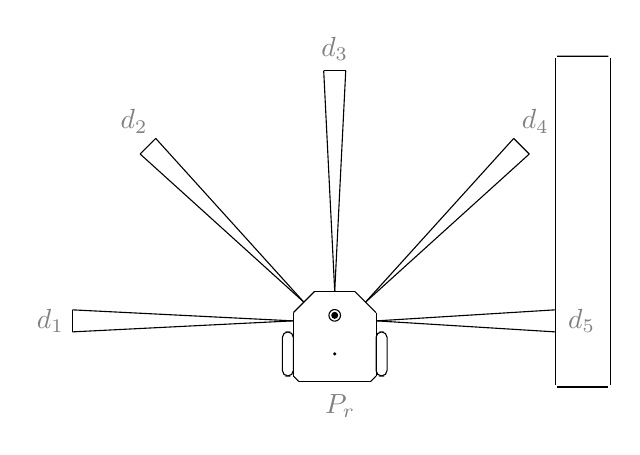
\begin{tikzpicture}[scale = 1.4]%
			\meuRoboLindaoCompEO
			\desenharSensoresTriangulo
		\end{tikzpicture}%
		
		\label{fig:CompEOa}%
		\caption{Sensores infravermelho}%
	\end{subfigure}%
	~
	\begin{subfigure}[t]{0.5\textwidth}%
		\centering%
		
		\begin{tikzpicture}[scale = 1.4]%
			\meuRoboLindaoCompEO
			\desenharSensoresVetores
		\end{tikzpicture}%
			
		\label{fig:CompEOb}%
		\caption{Vetores utilizados}%
	\end{subfigure}%
	\\
	\textbf{Fonte: autoria própria}
\end{figure}
		
		\subsubsection{Comportamento mesclado ''Ir Para Objetivo e Evitar Obstáculo''}
		
		\subsubsection{Mínimos locais}
		
		\newcommand{\meuRoboLindaoCompMinimos}{
	\begin{scope}[shift={(0,0.3)}]
		% Pr 
		\begin{scope}[shift={(0,-0.3)}, scale = 0.5]
			\node[color = gray] at (0.1,-0.35) {$P_r$};
		\end{scope}
		\begin{scope}[rotate=90,scale=0.5]
			\filldraw (0,0) circle (0.5pt);
			\begin{scope}[shift={(0.25,0)},rotate = -90]
				\RoboDiffClean
			\end{scope}
		\end{scope}
	\end{scope}
}%

\newcommand{\obstaculoA}[2]{
	\node[inner sep = 0pt] (P1) at (#1,0) {};
	\node[inner sep = 0pt] (P2) at (\fpeval{#1+(#2/2)},\fpeval{#2*sqrt{2}/2}) {};
	\node[inner sep = 0pt] (P3) at (\fpeval{#1+((3*#2)/2)},\fpeval{#2*sqrt{2}/2}) {};
	\node[inner sep = 0pt] (P4) at (\fpeval{#1+2*#2},0) {};
	\node[inner sep = 0pt] (P5) at (\fpeval{#1+((3*#2)/2)},\fpeval{-(#2*sqrt{2}/2)}) {};
	\node[inner sep = 0pt] (P6) at (\fpeval{#1+(#2/2)},\fpeval{-(#2*sqrt{2}/2)}) {};
	
	\draw[color = darkgray] (P1) -- (P2);
	\draw[color = darkgray] (P2) -- (P3);
	\draw[color = darkgray] (P3) -- (P4);
	\draw[color = darkgray] (P4) -- (P5);
	\draw[color = darkgray] (P5) -- (P6);
	\draw[color = darkgray] (P6) -- (P1);
	
	\node[color = gray] at (#1+#2,-1.3) {Obstáculo 1};
}

\newcommand{\obstaculoB}[3]{
	\node[inner sep = 0pt] (P1) at (#1,#2) {};
	\node[inner sep = 0pt] (P2) at (#1,#2+0.5) {};
	\node[inner sep = 0pt] (P3) at (#1+#3+0.5,#2+0.5) {};
	\node[inner sep = 0pt] (P4) at (#1+#3+0.5,-#2-0.5) {};
	
	\node[inner sep = 0pt] (P5) at (#1,-#2-0.5) {};
	\node[inner sep = 0pt] (P6) at (#1,-#2) {};
	\node[inner sep = 0pt] (P7) at (#1+#3,-#2) {};
	\node[inner sep = 0pt] (P8) at (#1+#3,#2) {};
	
	\draw[color = darkgray] (P1) -- (P2);
	\draw[color = darkgray] (P2) -- (P3);
	\draw[color = darkgray] (P3) -- (P4);
	\draw[color = darkgray] (P4) -- (P5);
	\draw[color = darkgray] (P5) -- (P6);
	\draw[color = darkgray] (P6) -- (P7);
	\draw[color = darkgray] (P7) -- (P8);
	\draw[color = darkgray] (P8) -- (P1);
	
	\node[color = gray] at (#1+0.25+#3/2,-2.8) {Obstáculo 2};
}

\newcommand{\obstaculoC}[2]{
	\node[inner sep = 0pt] (P1) at (#1,#2+0.5) {};
	\node[inner sep = 0pt] (P2) at (#1+0.5,#2+0.5) {};
	\node[inner sep = 0pt] (P3) at (#1+0.5,-#2-0.5) {};
	\node[inner sep = 0pt] (P4) at (#1,-#2-0.5) {};
	
	\draw[color = darkgray] (P1) -- (P2);
	\draw[color = darkgray] (P2) -- (P3);
	\draw[color = darkgray] (P3) -- (P4);
	\draw[color = darkgray] (P4) -- (P1);
	
	\node[color = gray] at (#1+0.25,-2.8) {Obstáculo 3};
}

\begin{figure}[ht]
	\centering%
	\caption{Tipos de obstáculos}%
	\label{fig:CompSP}%
		
	\begin{tikzpicture}[scale = 1.4]%
		% Robô
		\begin{scope}[rotate=-90]
			\meuRoboLindaoCompMinimos
		\end{scope}
		\obstaculoA{2}{1.5}
		\obstaculoB{4}{2}{2}
		\obstaculoC{8}{2}
		
		\begin{scope}[shift={(10,0)}]
			\filldraw (0,0) circle (1.5pt);
			\node[color = gray] at (0,-0.35) {Objetivo};
		\end{scope}
	\end{tikzpicture}%

	\textbf{Fonte: autoria própria}
\end{figure}
		
		\subsubsection{Comportamento ''Seguir parede''}
		
		\newcommand{\meuRoboLindaoCompSP}{
	\begin{scope}[shift={(0,0.3)}]
		% Pr 
		\begin{scope}[shift={(0,-0.3)}, scale = 0.5]
			\node[color = gray] at (0.1,-0.35) {$P_r$};
		\end{scope}
		\begin{scope}[rotate=90,scale=0.5]
			\filldraw (0,0) circle (0.5pt);
			\begin{scope}[shift={(0.25,0)},rotate = -90]
				\RoboDiffClean
			\end{scope}
		\end{scope}
	\end{scope}
}%

\newcommand{\parede}[2]{
	\node[inner sep = 0pt] (P1) at (0,0) {};
	\node[inner sep = 0pt] (P2) at (#2,0) {};
	\node[inner sep = 0pt] (P3) at (#2,0.5) {};
	\node[inner sep = 0pt] (P4) at (0.5,0.5) {};
	\node[inner sep = 0pt] (P5) at (0.5,#1) {};
	\node[inner sep = 0pt] (P6) at (0,#1) {};
	\draw[color = darkgray] (P1) -- (P2);
	\draw[color = darkgray] (P2) -- (P3);
	\draw[color = darkgray] (P3) -- (P4);
	\draw[color = darkgray] (P4) -- (P5);
	\draw[color = darkgray] (P5) -- (P6);
	\draw[color = darkgray] (P6) -- (P1);
}

\newcommand{\sensorVisaoTriangularSp}[1]{
	\draw[color = gray] (0,0) -- (-0.1,#1);
	\draw[color = gray] (0,0) -- (0.1,#1);
	\draw[color = gray] (-0.1,#1) -- (0.1,#1);
}

\newcommand{\sensorVisaoVetorSp}[1]{
	\draw[->] (0,0) -- (0,#1);
}

\newcommand{\desenharSensoresTrianguloSPa}{
	\begin{scope}[shift={(0.38,0.6)},rotate=-90]
		\sensorVisaoTriangularSp{2}
	\end{scope}
	\begin{scope}[shift={(-0.38,0.6)},rotate=90]
		\sensorVisaoTriangularSp{2-1.3}
	\end{scope}
	\begin{scope}[shift={(0.28,0.77)},rotate=-45]
		\sensorVisaoTriangularSp{2}
	\end{scope}
	\begin{scope}[shift={(-0.28,0.77)},rotate=45]
		\sensorVisaoTriangularSp{2}
	\end{scope}	
	\begin{scope}[shift={(0,0.87)},rotate=0]
		\sensorVisaoTriangularSp{2}
	\end{scope}
}

\newcommand{\desenharSensoresTrianguloSPb}{
	\begin{scope}[shift={(0.38,0.6)},rotate=-90]
		\sensorVisaoTriangularSp{2-0.9}
	\end{scope}
	\begin{scope}[shift={(-0.38,0.6)},rotate=90]
		\sensorVisaoTriangularSp{2}
	\end{scope}
	\begin{scope}[shift={(0.28,0.77)},rotate=-45]
		\sensorVisaoTriangularSp{2-0.5}
	\end{scope}
	\begin{scope}[shift={(-0.28,0.77)},rotate=45]
		\sensorVisaoTriangularSp{2}
	\end{scope}	
	\begin{scope}[shift={(0,0.87)},rotate=0]
		\sensorVisaoTriangularSp{2-1}
	\end{scope}
}

\newcommand{\desenharLinhasParedeA}{
	\begin{scope}[shift={(-0.38,0.6)},rotate=90]
		\begin{scope}[shift={(0,2-1.3)}]
			\node[inner sep = 0pt] (P1) at (0,0) {};
		\end{scope}
	\end{scope}
	\begin{scope}[shift={(-0.28,0.77)},rotate=45]
		\begin{scope}[shift={(0,2)}]
			\node[inner sep = 0pt] (P2) at (0,0) {};
		\end{scope}
	\end{scope}
	
	\draw (P1) -- (P2);
}

\newcommand{\desenharLinhasParedeB}{
	\begin{scope}[shift={(0.38,0.6)},rotate=-90]
		\begin{scope}[shift={(0,2-0.9)}]
			\node[inner sep = 0pt] (P1) at (0,0) {};
		\end{scope}
	\end{scope}
	\begin{scope}[shift={(0,0.87)},rotate=0]
		\begin{scope}[shift={(0,2-1)}]
			\node[inner sep = 0pt] (P2) at (0,0) {};
		\end{scope}
	\end{scope}
	
	\draw (P1) -- (P2);
}

\begin{figure}[ht]
	\centering%
	\caption{Comportamento Seguir Parede}%
	\label{fig:CompSP}%
	\begin{subfigure}[t]{0.5\textwidth}%
		\centering%
		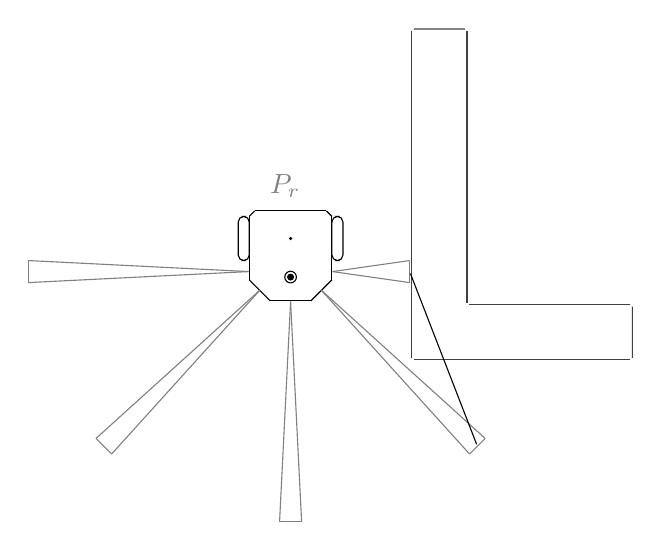
\begin{tikzpicture}[scale = 1.4]%
			% Obstáculo
			\parede{3}{2}
			% Robô
			\begin{scope}[shift={(-1.1,1.4)},rotate=180]
				\meuRoboLindaoCompSP
				\desenharSensoresTrianguloSPa
				\desenharLinhasParedeA
			\end{scope}
		\end{tikzpicture}%
		
		\label{fig:CompSPa}%
		\caption{Parede subestimada}%
	\end{subfigure}%
	~
	\begin{subfigure}[t]{0.5\textwidth}%
		\centering%
		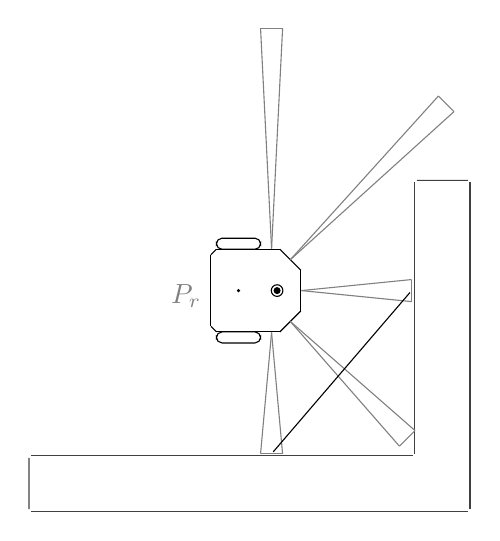
\begin{tikzpicture}[scale = 1.4]%
			% Obstáculo
			\begin{scope}[shift={(0,0)},xscale=-1,yscale=1]
				\parede{3}{4}
			\end{scope}
			% Robô
			\begin{scope}[shift={(-2.4,2)},rotate=-90]
				\meuRoboLindaoCompSP
				\desenharSensoresTrianguloSPb
				\desenharLinhasParedeB
			\end{scope}
		\end{tikzpicture}%
			
		\label{fig:CompSPb}%
		\caption{Parede superestimada}%
	\end{subfigure}%
	\\
	\textbf{Fonte: autoria própria}
\end{figure}
		
		\newcommand{\desenharLinhasParedeC}[2]{
	\begin{scope}[shift={(-0.38,0.6)},rotate=90]
		\begin{scope}[shift={(0,2-1.3)}]
			\node[inner sep = 0pt] (P1) at (0,0) {};
		\end{scope}
	\end{scope}
	\begin{scope}[shift={(-0.28,0.77)},rotate=45]
		\begin{scope}[shift={(0,2)}]
			\node[inner sep = 0pt] (P2) at (0,0) {};
		\end{scope}
	\end{scope}
	
	\draw (P1) -- (P2);
	
	% linhas continuacao:
	\def\UserVetAX{-1.08}
	\def\UserVetAY{0.6}
	
	\def\UserVetXNum{\fpeval{-0.28-sqrt(2)+1.08}}
	\def\UserVetYNum{\fpeval{0.77+sqrt(2)-0.6}}
	\def\UserVetMod{\fpeval{sqrt(\UserVetXNum*\UserVetXNum + \UserVetYNum*\UserVetYNum)}}
	
	\def\UserVetX{\fpeval{\UserVetXNum/\UserVetMod}}
	\def\UserVetY{\fpeval{\UserVetYNum/\UserVetMod}}
	
	\def\UserLinhaTrasX{\fpeval{-1.08 -\UserVetX*#1}}
	\def\UserLinhaTrasY{\fpeval{0.6 -\UserVetY*#1}}
	\def\UserLinhaFrenteX{\fpeval{-0.28-sqrt(2) +\UserVetX*#2}}
	\def\UserLinhaFrenteY{\fpeval{0.77+sqrt(2) +\UserVetY*#2}}
			
	\draw [dashed] (P1) -- (\UserLinhaTrasX,\UserLinhaTrasY);
	\draw [dashed] (P2) -- (\UserLinhaFrenteX,\UserLinhaFrenteY);
	
	\def\distance{\fpeval{\UserVetX * \UserVetAX + \UserVetY * (\UserVetAY - 0.3)}}
	\begin{scope}[shift={(0,0.3)}]
		\def\UserVetPerpX{\fpeval{\UserVetAX-\distance*\UserVetX}}
		\def\UserVetPerpY{\fpeval{(\UserVetAY - 0.3)-\distance*\UserVetY}}
		\def\UserVetPerpNormX{\UserVetPerpX/(sqrt(\UserVetPerpX*\UserVetPerpX + \UserVetPerpY*\UserVetPerpY))}
		\def\UserVetPerpNormY{\UserVetPerpY/(sqrt(\UserVetPerpX*\UserVetPerpX + \UserVetPerpY*\UserVetPerpY))}
	
		\draw[-{Latex[length=2mm]}] (0,0) -- (P1) node [black,midway,yshift=-0.21cm,xshift=0.1cm] {$u_a$};
		\begin{scope}[shift={(P1)}]
			\draw[-{Latex[length=2mm]}] (0,0) -- (\UserVetX, \UserVetY) node [black,midway,xshift=-0.3cm,yshift=0.1cm] {$u_t$};
		\end{scope}
		\draw[-{Latex[length=2mm]}] (0,0) -- (\UserVetPerpX, \UserVetPerpY)
		node [black,midway,yshift=0.3cm,xshift=0.2] {$u_p$};

		\def\UserChavesX{\fpeval{\UserVetAX-\distance*\UserVetX}}
		\def\UserChavesY{\fpeval{(\UserVetAY - 0.3)-\distance*\UserVetY}}	
		\draw [decorate,decoration={brace,amplitude=10pt},xshift=-2pt,yshift=-2pt]
			(\UserChavesX, \UserChavesY) -- (\fpeval{-1.08},\fpeval{0.3}) 
			node [black,midway,xshift=0.6cm, yshift=0.1cm] {$d$};
			
		% angulo reto:
		\def\UserTamanhoQuad{0.15}
		\def\UserPontoEsqX{\fpeval{\UserVetPerpX - \UserTamanhoQuad*\UserVetPerpNormX}}
		\def\UserPontoEsqY{\fpeval{\UserVetPerpY - \UserTamanhoQuad*\UserVetPerpNormY}}
		\def\UserPontoDirX{\fpeval{\UserVetPerpX + \UserTamanhoQuad*\UserVetX}}
		\def\UserPontoDirY{\fpeval{\UserVetPerpY + \UserTamanhoQuad*\UserVetY}}
		\def\UserPontoBaixoX{\fpeval{\UserVetPerpX - \UserTamanhoQuad*\UserVetPerpNormX + \UserTamanhoQuad*\UserVetX}}
		\def\UserPontoBaixoY{\fpeval{\UserVetPerpY - \UserTamanhoQuad*\UserVetPerpNormY + \UserTamanhoQuad*\UserVetY}}
		
		\draw (\UserVetPerpX, \UserVetPerpY) -- (\UserPontoEsqX, \UserPontoEsqY);
		\draw (\UserVetPerpX, \UserVetPerpY) -- (\UserPontoDirX, \UserPontoDirY);
		\draw (\UserPontoEsqX, \UserPontoEsqY) -- (\UserPontoBaixoX, \UserPontoBaixoY);
		\draw (\UserPontoDirX, \UserPontoDirY) -- (\UserPontoBaixoX, \UserPontoBaixoY);
		
		\filldraw (\fpeval{\UserVetPerpX - \UserTamanhoQuad*\UserVetPerpNormX/2 + \UserTamanhoQuad*\UserVetX/2}, 
		\fpeval{\UserVetPerpY - \UserTamanhoQuad*\UserVetPerpNormY/2 + \UserTamanhoQuad*\UserVetY/2}) circle (0.5pt);
		
		% Ângulo vetor
		\begin{scope}[shift={(P1)}, rotate=180]
			\draw (0.3*\UserVetX,0.3*\UserVetY) arc (110:160:0.3);
			\node at (-0.35,0.25) {\footnotesize $\theta$};
		\end{scope}
	\end{scope}
}

\begin{figure}[ht]
	\centering%
	\caption{Recomendação vetorial}%
	\label{fig:CompSPVetor}%
	
	\begin{tikzpicture}[scale = 1.4]%
		% Obstáculo
		%\parede{3}{2}
		% Robô
		\begin{scope}[shift={(-1.1,1.4)},rotate=180]
			\meuRoboLindaoCompSP
			\desenharSensoresTrianguloSPa
			\desenharLinhasParedeC{3}{2}
		\end{scope}
	\end{tikzpicture}%
	\\
	\textbf{Fonte: autoria própria}
\end{figure}
		
		\begin{equation}
			\label{eq:vetorPerpendicularSP1}
			\mathbf{u_a} \cdot \mathbf{u_t} = \mid \mathbf{u_a} \mid \cdot \mid \mathbf{u_t} \mid \cos(\theta)
		\end{equation}
		
		\begin{equation}
			\label{eq:vetorPerpendicularSP2}
			\mathbf{u_a} \cdot \mathbf{u_t} = \mid \mathbf{u_a} \mid \cos(\theta) = d
		\end{equation}
		
		\begin{equation}
			\label{eq:vetorPerpendicularSP3}
			\mathbf{u_p} = \mathbf{u_a} - d \cdot \mathbf{u_t}
		\end{equation}
		
		\subsubsection{O autômato para arbitragem de comportamentos}
	
		\tikzset{%
    block/.style={draw, fill=white, rectangle, 
            minimum height=2em, minimum width=3em},
    input/.style={inner sep=0pt},       
    output/.style={inner sep=0pt},      
    sum/.style = {draw, fill=white, circle, minimum size=2mm, node distance=1.5cm, inner sep=0pt},
    pinstyle/.style = {pin edge={to-,thin,black}}
}

\newcommand{\automatoHibrido}[1]{
\begin{tikzpicture}[scale = 1.1,->,auto ,node distance =4 cm and 5cm , on grid,
>=latex ,
state/.style ={scale = 1.1, circle, draw, minimum width =0.7cm},
finalstate/.style ={scale = 1.1, circle, draw, minimum width =0.7cm}]

	\node[state] (No3) {3};
	\begin{scope}[rotate=90]
		\begin{scope}[shift={(#1,0)}]
			\node[state] (No0) {0};
		\end{scope}
	\end{scope}
	\begin{scope}[rotate=90-72]
		\begin{scope}[shift={(#1,0)}]
			\node[state] (No5) {5};
		\end{scope}
	\end{scope}
	\begin{scope}[rotate=90-72*2]
		\begin{scope}[shift={(#1,0)}]
			\node[state] (No2) {2};
		\end{scope}
	\end{scope}
	\begin{scope}[rotate=90-72*3]
		\begin{scope}[shift={(#1,0)}]
			\node[state] (No1) {1};
		\end{scope}
	\end{scope}
	\begin{scope}[rotate=90-72*4]
		\begin{scope}[shift={(#1,0)}]
			\node[state] (No4) {4};
		\end{scope}
	\end{scope}
	
	\path[->] (No4) edge[bend left=20] node[xshift=-1cm, yshift=0.2cm] {$\neg a \land b \land \neg f$} (No3);
	\path[->] (No3) edge[bend left=20] node[xshift=1cm, yshift=-0.2cm] {$\neg a \land \neg b \land f$} (No4);
	\path[->] (No3) edge[bend left=20] node[xshift=1cm, yshift=0.2cm] {$\neg a \land \neg b \land g$} (No5);
	\path[->] (No5) edge[bend left=20] node[xshift=-0.1cm] {$\neg a \land b \land \neg g$} (No3);
	\path[->] (No3) edge[bend left=20] node[xshift=-0.9cm, yshift=1cm, rotate=-45] {$\neg a \land b \land \neg e \land d$} (No2);
	\path[->] (No2) edge[bend left=20] node[xshift=0.5cm, yshift=-0.6cm, rotate=-45] {$\neg a \land \neg d$} (No3);
	\path[->] (No3) edge[bend left=20] node {$a$} (No0);
	\path[->] (No0) edge[bend left=20] node {$\neg a$} (No3);
	\path[->] (No3) edge[bend left=20] node[xshift=-0.5cm, yshift=-0.6cm, rotate=45] {$\neg a \land b \land e$} (No1);
	\path[->] (No1) edge[bend left=20] node[xshift=0.2cm, yshift=0.3cm, rotate=45] {$\neg a \land b \land c$} (No3);
	
	\path[->] (No1) edge node {$\neg a \land b \land \neg c \land d$} (No2);
	\path[->] (No1) edge node[xshift=2.4cm, yshift=0.8cm] {$\neg a \land \neg b \land f$} (No4);
	\path[->] (No4) edge node {$a$} (No0);
	\path[->] (No5) edge node {$a$} (No0);
	
	\path[->,draw] (No1) .. controls ($(No2)+(1.5,-2)$) .. node[yshift=-0.2cm] {$\neg a \land \neg b \land g$} (No5);
	\path[->,draw] (No1) .. controls ($(No4)+(-2,1)$) .. node {$a$} (No0);
	\path[->,draw] (No2) .. controls ($(No5)+(2.1,1)$) .. node {$a$} (No0);
	
	% Input
	\coordinate[above = 1cm of No0, inner sep = 0pt] (input) {};
	\path[->] (input) edge (No0);
	
\end{tikzpicture}%
}

% Figura
\begin{figure}[ht]
	\centering
	\caption{Autômato Híbrido que soluciona o problema de navegação} 
	\label{fig:automatoHibrido}

	\automatoHibrido{5}
		
	\textbf{Fonte: autoria própria}
\end{figure}
	
		\begin{table}[ht]
\centering
\caption{Estados do autômato}
\vspace{0.2 cm}
\begin{tabular}{|c|l|l|}
\hline
Índice & Comportamento & Descrição                                         \\ \hline
0      & P             & Parar                                             \\ \hline
1      & IPO           & Ir para Objetivo                                  \\ \hline
2      & EO            & Evitar Obstáculos                                 \\ \hline
3      & IPO\_E\_EO    & Ir para Objetivo e Evitar Obstáculos (combinados) \\ \hline
4      & SP AH         & Seguir Parede sentido Anti-horário				   \\ \hline
5      & SP H          & Seguir Parede sentido Horário                     \\ \hline
\end{tabular}
\label{tab:automatoEstados}
\end{table}
		
		\begin{table}[ht]
\centering
\caption{Condições utilizadas nas transições do autômato}
\vspace{0.2 cm}
\begin{tabular}{|c|l|l|}
\hline
Legenda & Condições                 & Cálculo da condição \\ \hline
a       & No objetivo               & Equacao1            \\ \hline
b       & Fez progresso             & Equacao1            \\ \hline
c       & Tem Obstáculo             & Equacao1            \\ \hline
d       & Está inseguro             & Equacao1            \\ \hline
e       & Livre de obstáculo        & Equacao1            \\ \hline
f       & Contornando pela esquerda & Equacao1            \\ \hline
g       & Contornando pela direita  & Equacao1            \\ \hline
\end{tabular}
\label{tab:automatoEventos}
\end{table}
	
	\subsection{Por Controlador \textit{Fuzzy}}
	
	Nesta seção, pretende-se demonstrar um controlador simples capaz de solucionar 
	o problema de navegação, usando sistema \textit{fuzzy}.
	
	\subsubsection{Comportamento ''Gerar Recomendação''}
	
	a
	
	\subsubsection{Comportamento ''Seguir parede''}
	
	\subsubsection{Comportamento ''Seguir Recomendação''}
	
	\subsubsection{A estratégia para fusão de comportamentos}
	
\section{Simulação}

	\subsection{Utilizando controlador Híbrido}
	
	a
	
	\subsection{Utilizando controlador \textit{Fuzzy}}
	
	a
	
\section{Montagem Física}

	\subsection{Processo de montagem}

	\subsection{Curvas dos motores}

a
	
\section{Implementação do sistema embarcado}

	\subsection{Considerações práticas, limitações do modelo e da simulação}

	\subsection{Esquema lógico do sistema embarcado}

	\subsection{Projeto da placa}
	
	a
	
	\subsection{Implementação da abordagem Híbrida}

	\subsection{Implementação da solução \textit{Fuzzy}}
	
\section{Resultado e Discussão}

	\subsection{Resultado para contrador híbrido}

	a
	
	\subsection{Resultado para contrador \textit{fuzzy}}

\chapter{Considerações Finais}
\vspace{-2.5 cm}

Para concluir esta etapa do trabalho, algumas deliberações precisam ser feitas.
Por enquanto, uma parte do trabalho foi completamente desconsiderada: estimativa
do estado do sistema. Para simulação, muitos trabalhos acadêmicos consideram o
estado atual do robô como um valor conhecido. Para um robô real, autônomo, este
estado pode ser estimado usando técnicas como observadores, filtro de Kalman,
odometria, entre outras.

É importante salientar que há um conflito entre os objetivos deste trabalho,
já que um robô ao mesmo tempo autônomo e sem armazenamento de mapa deve possuir
a capacidade de estimar com perfeição seu estado atual. Na prática, a estimativa
de estado carrega erros que são somados no decorrer do tempo de execução. Para
corrigir tais erros, ou o robô deve armazenar mapa (representação interna do
mundo à sua volta) e reconhecer locais já visitados, ou o robô precisa de um
sistema externo (computador com câmera, sistema GPS) que envie correções
(isso reduz autonomia). 

A segunda solução pode ser adotada neste trabalho, a fim de torná-lo mais focado
no aspecto de controle e navegação, o que possibilitará explorar as diferentes
abordagens estipuladas (controle híbrido e \textit{fuzzy}) com maior
aproveitamento. 

Desta forma, uma comparação qualitativa será efetuada. Esta análise
deve ser qualitativa pois não existe um padrão de teste (\textit{benchmark})
amplamente adotado em robótica móvel. Logo, qualquer análise comparativa só pode
ser qualitativa.








% \section{Comandos latex (desconsiderar)}
% \begin{equation}
% 	^{A}P = _{B}^{A}R ^{B}P + ^{A}Q_{B_{origem}}
% 	\label{eq:trans} 
% \end{equation}
% 
% \begin{equation}
% 	^{A}P = _{B}^{A}T ^{B}P = \mleft[
% 	\begin{array}{c|c}
% 		  _{B}^{A}R & ^{A}Q_{B_{Origem}} \\
% 			  \hline
% 		  0 \quad 0 \quad 0 & 1
% 	\end{array}
% 	\mright] \mleft[ 
% 	\begin{array}{c c}
% 	^{B}P_{x} \\ ^{B}P_{y} \\ ^{B}P_{z} \\ 1
% 	\end{array}
% 	\mright] = \mleft[
% 	\begin{matrix}
% 		  _{B}^{A}R_{11} & _{B}^{A}R_{12} & _{B}^{A}R_{13} & Q_{x} \\
% 		  _{B}^{A}R_{21} & _{B}^{A}R_{22} & _{B}^{A}R_{23} & Q_{y} \\
% 		  _{B}^{A}R_{31} & _{B}^{A}R_{32} & _{B}^{A}R_{33} & Q_{z} \\
% 		  0 & 0 & 0 & 1
% 	\end{matrix}
% 	\mright] \mleft[ 
% 	\begin{array}{c c}
% 	^{B}P_{x} \\ ^{B}P_{y} \\ ^{B}P_{z} \\ 1
% 	\end{array}
% 	\mright]
% \end{equation} 
% 
% \begin{equation}
% 	_{B}^{A}T^{-1} = _{A}^{B}T = \mleft[
% 	\begin{array}{c|c}
% 		  _{B}^{A}R^{T} & -_{B}^{A}R^{T} \: ^{A}Q_{B_{Origem}} \\
% 		  \hline
% 		  0 \quad 0 \quad 0 & 1
% 	\end{array}
% 	\mright]
% \end{equation}